%----------------------------------------------------------------------------------------
%	PACKAGES AND THEMES
%----------------------------------------------------------------------------------------
\PassOptionsToPackage{table}{xcolor}
\documentclass[aspectratio=169,xcolor=dvipsnames,svgnames,x11names,fleqn]{beamer}
% \documentclass[aspectratio=169,xcolor=dvipsnames,fleqn]{beamer}

\usetheme{RedVelvet}

\usefonttheme[onlymath]{serif}
\newcommand{\showanswers}{yes}


\usepackage{xspace}
\usepackage{amsmath}
\usepackage{amssymb}
\usepackage{amsfonts}
\usepackage{color}
\usepackage{physics}
% \usepackage{mathbb}
\usepackage{rahul_math}
\usepackage{bigints}

\usepackage{graphicx} % Allows including images
\usepackage{booktabs} % Allows the use of \toprule, \midrule and \bottomrule in tables
\usepackage{tikz,pgfplots}

\usepackage{subfigure}
\usetikzlibrary{arrows}
\usepackage{minted}
\definecolor{LightGray}{gray}{0.9}
\definecolor{cream}{rgb}{0.92, 0.9, 0.55}
\definecolor{lightblue}{rgb}{0.68, 0.85, 0.9}


\usepackage{xcolor-material}
\usetikzlibrary{fit}
\usetikzlibrary{matrix}
\tikzset{%
apple/.pic={
    \fill [MaterialBrown] (-1/8,0)  arc (180:120:1 and 3/2) coordinate [pos=3/5] (@)-- ++(1/6,-1/7)  arc (120:180:5/4 and 3/2) -- cycle;
    \fill [MaterialLightGreen500] (0,-9/10)  .. controls ++(180:1/8) and ++(  0:1/4) .. (-1/3,  -1) .. controls ++(180:1/3) and ++(270:1/2) .. (  -1,   0) .. controls ++( 90:1/3) and ++(180:1/3) .. (-1/2, 3/4) .. controls ++(  0:1/8) and ++(135:1/8) .. (   0, 4/7)
    }
    }

\newcommand{\leftdoublequote}{\textcolor{blue}{\scalebox{3}{``}}}

\newcommand{\rightdoublequote}{\textcolor{blue}{\scalebox{3}{''}}}


\usepackage{textcomp}
\usepackage{fontawesome}
\usepackage{tikz,pgfplots}
\usetikzlibrary{shapes.callouts}
\usetikzlibrary{arrows}


\usepackage{overpic}

%----------------------------------------------------------------------------------------
%	TITLE PAGE
%----------------------------------------------------------------------------------------

\usepackage{tikz-qtree,tikz-qtree-compat}
\usetikzlibrary{tikzmark}
\usetikzlibrary{calc}


\title[CPE 486/586: Machine Learning]{CPE 486/586: Machine Learning for Engineers} % The short title appears at the bottom of every slide, the full title is only on the title page
\subtitle{06 Linear Regression}

\author[Rahul Bhadani] {{\Large \textbf{Rahul Bhadani}}}

\institute[UAH] % Your institution as it will appear on the bottom of every slide, maybe shorthand to save space
{
    Electrical \& Computer Engineering,  The University of Alabama in Huntsville
}
\date

% \titlegraphic{
%    \includegraphics[width=0.4\linewidth]{figures/UAH_primary.png}
% }

\begin{document}

%-------------------------------------------------
\begin{frame}
    \titlepage
\end{frame}

%-------------------------------------------------
\begin{frame}{Outline}
    \backgroundtableofcontents
\end{frame}



  

%%%%%%%%%%%%%%%%%%%%%%%%%%%%%%%%%%%%%%%%%%%%%%%%%%%%%
\begin{sectionframe}{\faKeyboardO}{Machine Learning}
\end{sectionframe}


\begin{frame}{What is Machine Learning?}

    \begin{columns}
        \column{0.5\linewidth}
        \begin{center}
            \Large
            Give a computer ability to learn without explicit programming using data.
        \end{center}
        \column{0.5\linewidth}
        \begin{center}
            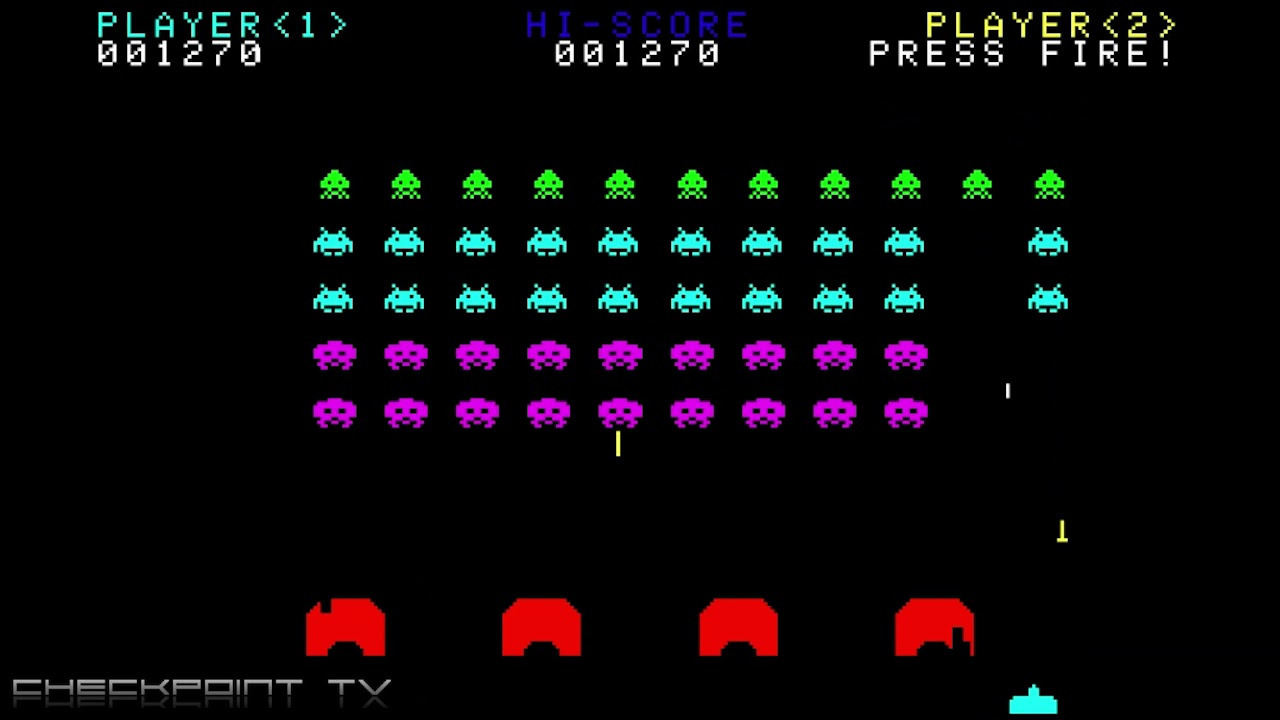
\includegraphics[width=0.8\linewidth]{figures/atari.jpg}
        \end{center}
    \end{columns}
\end{frame}

\begin{frame}{Supervised vs Unsupervised Learning}

    \begin{columns}
        \column{0.5\linewidth}
        \begin{center}
            \textbf{Supervised Learning}

            \begin{itemize}
                \item Input ($\xbf$) and output label $y$ data available.
                \item We learn a mapping $f: \xbf \to y$.
                \item Give a learnt mapping $f$ and a new $\xbf$, a computer can guess $y$.
            \end{itemize} 

        \end{center}
        \column{0.5\linewidth}
        \begin{center}
            \textbf{Unsupervised Learning}   
            \begin{itemize}
                \item Only Input ($\xbf$) data available.
                \item Uncover patterns.
                \item Learn to distinguish $\xbf_1$ from $\xbf_2$.
            \end{itemize}

        \end{center}
    \end{columns}

\end{frame}

%%%%%%%%%%%%%%%%%%%%%%%%%%%%%%%%%%%%%%%%%%%%%%%%%%%%%
\begin{sectionframe}{\faAreaChart}{Supervised Learning}
\end{sectionframe}

\begin{frame}{What is Supervised Learning}
    \begin{center}

            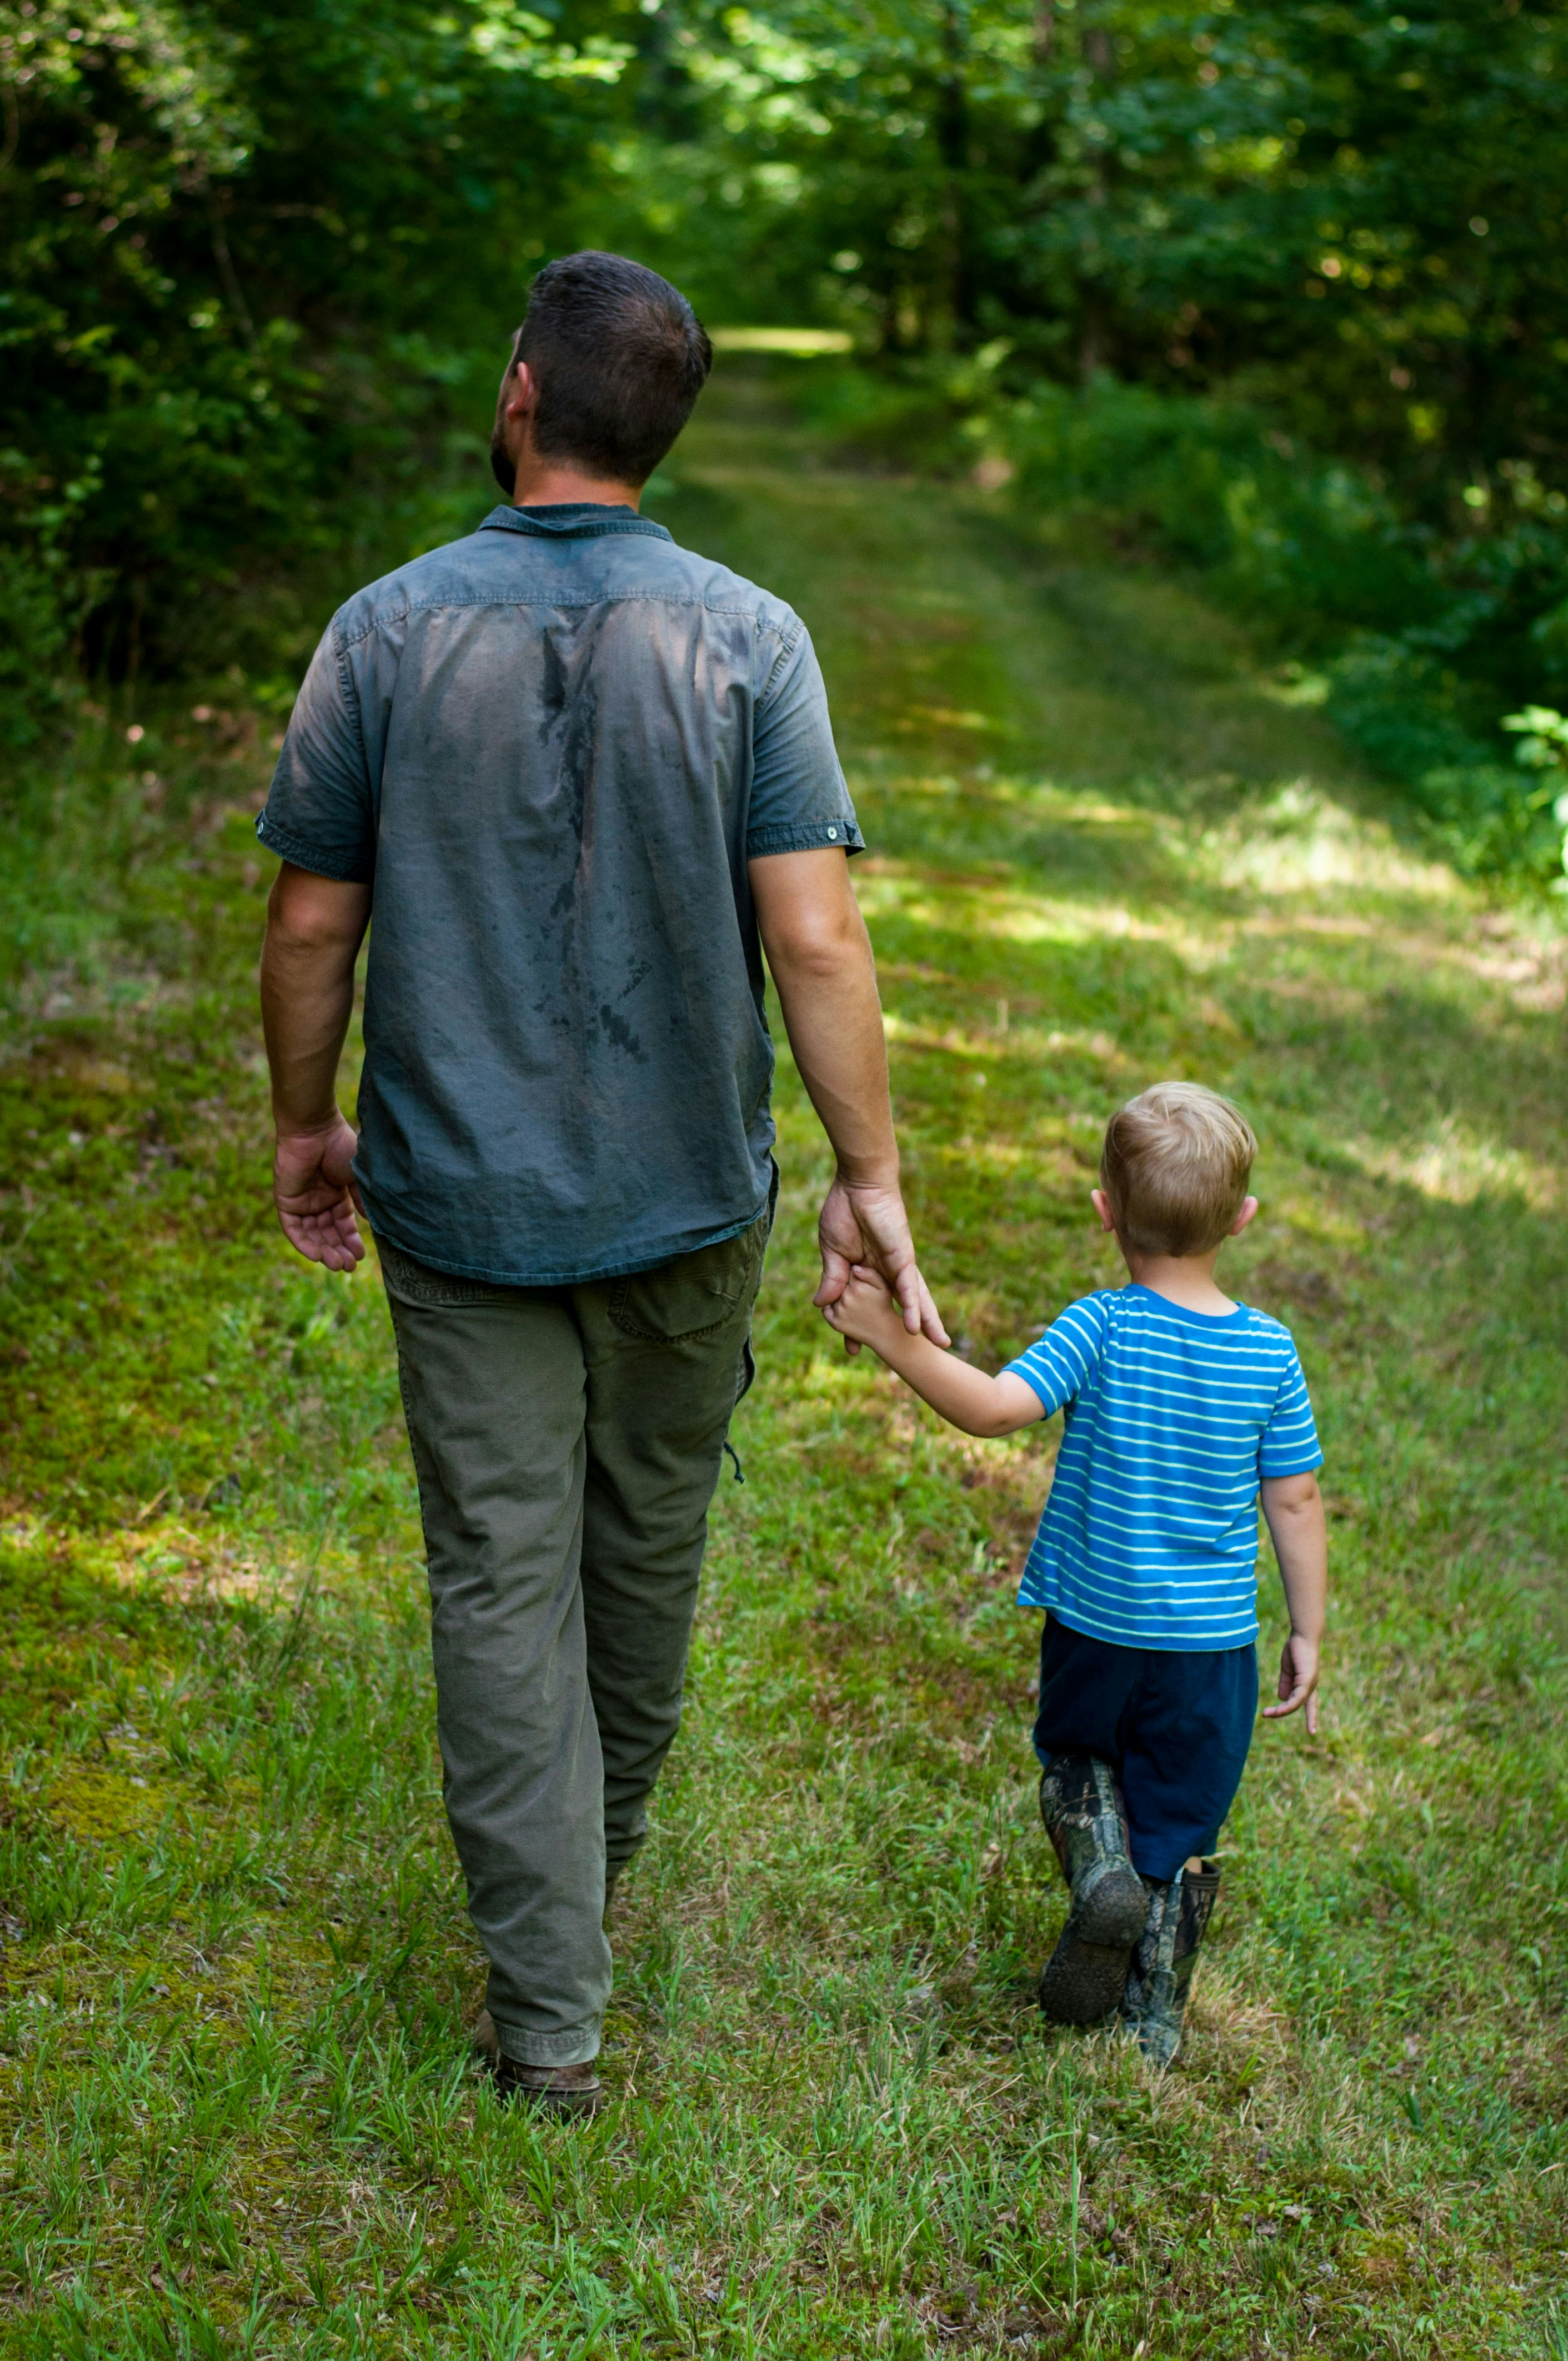
\includegraphics[width=0.2\linewidth]{figures/supervision.jpg}

            Learn from examples

    \end{center}
\end{frame}

\begin{frame}{Supervised Learning from Examples}
\small
    \begin{tabular}{p{0.25\textwidth} p{0.05\textwidth} p{0.25\textwidth}p{0.35\textwidth}}
        \textbf{Input $\xbf$} & &  \textbf{Output $y$} & \textbf{Application}\\
        \hline \\ 
        Email & $\to$ & Spam (? (0/1) ) & Spam Filtering\\ \\
        Audio & $\to$ & Text Transcripts & Speech Recognition\\ \\
        English & $\to$ & Bengali & Machine Translation\\ \\
        Ad, User Infor & $\to$ & Clicked (0/1) & Online Advertising \\ \\
        Image, Radar Info & $\to$ & Position of other Cards & Self-driving Cars \\ \\
        Image of Phone & $\to$ & Defect (0/1) & Automated Quality Inspection
        \end{tabular}
    
\end{frame}



\begin{frame}{The Supervised Learning Setting}

 \begin{itemize}
        \item Consider {\bf\color{MediumBlue}Input}: $\Dcal:=\{(\x_i, y_i)\}_{i=1}^n$ where $\xbf_i \in X$ is the feature vector (called \textbf{explanatory/predictor variable}), and $y_i \in Y$ is the known true label (called \textbf{response variable}). 
        \item Supervised learning algorithms learn from \underline{\textbf{``right answers"}}
    \end{itemize}

\end{frame}

\begin{frame}{Two Types of Supervised Learning}


    \begin{columns}
        \column{0.55\linewidth}
\begin{center}
    \large
    \textbf{1. Regression}

    \vspace{5pt}

    \hrulefill
    
    \vspace{15pt}

    \textbf{Input:} continuous/categorical data points (or a vector of data points)
    
    \vspace{10pt}

    \textbf{Output:} continuous data points (floating point real numbers)

    \vspace{10pt}

    \textbf{Example}: 
    Input: \{road curvature, traffic density, precipitation\}

    Output: Driving speed to the car.
    

\end{center}

\column{0.35\linewidth}

\includegraphics[width=0.9\linewidth]{figures/car.png}

\end{columns}
    
\end{frame}

\begin{frame}{Two Types of Supervised Learning}


    \begin{columns}
        \column{0.55\linewidth}
\begin{center}
    \large
    \textbf{2. Classification}

    \vspace{5pt}

    \hrulefill
    
    \vspace{15pt}

    \textbf{Input:} continuous/categorical data points  (or a vector of data points)
    
    \vspace{10pt}

    \textbf{Output:} categorical data points (also known as \textbf{class} or \textbf{category}) (yes/no, red/blue/green, defective/intact/partially defective)

    \vspace{10pt}

    \textbf{Example}: 
    Input: \{current speed of the car, LiDAR data\}

    Output: Moving Obstacle/Static Obstacle
    

\end{center}

\column{0.35\linewidth}
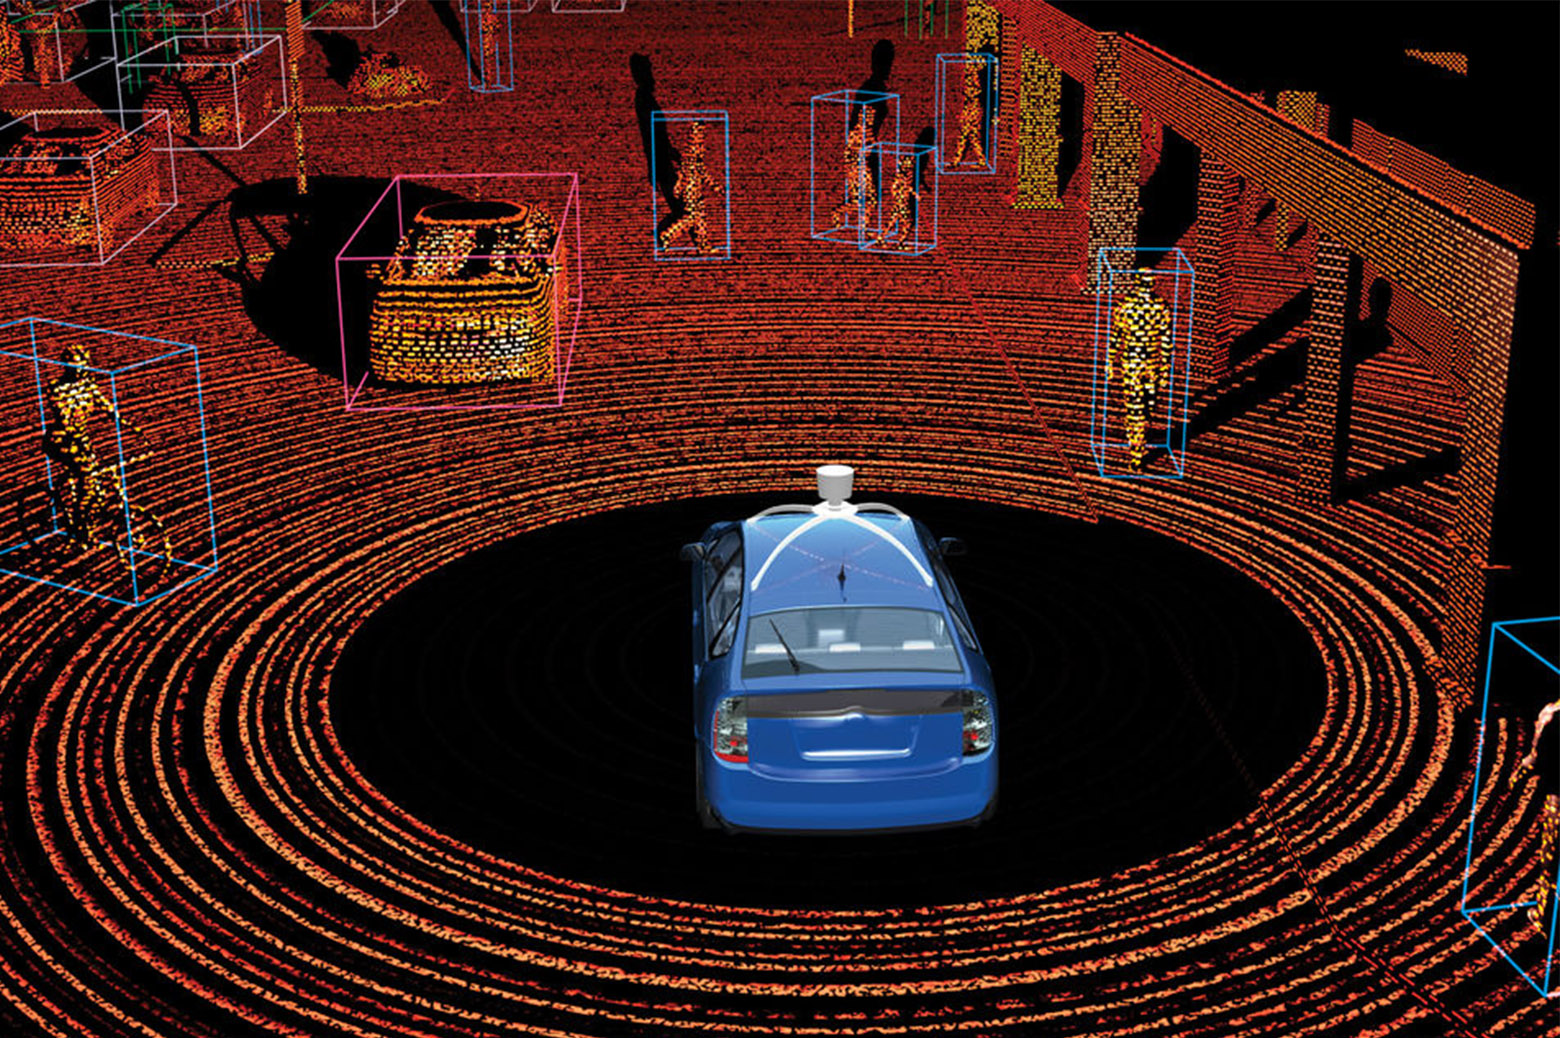
\includegraphics[width=0.9\linewidth]{figures/lidar-attack-content.jpg}

\end{columns}
    
\end{frame}

%%%%%%%%%%%%%%%%%%%%%%%%%%%%%%%%%%%%%%%%%%%%%%%%%%%%%
\begin{sectionframe}{\faLineChart}{Linear Regression}
\end{sectionframe}

\begin{frame}{References}

        \begin{columns}
            \column{0.95\linewidth}
            \begin{center}
        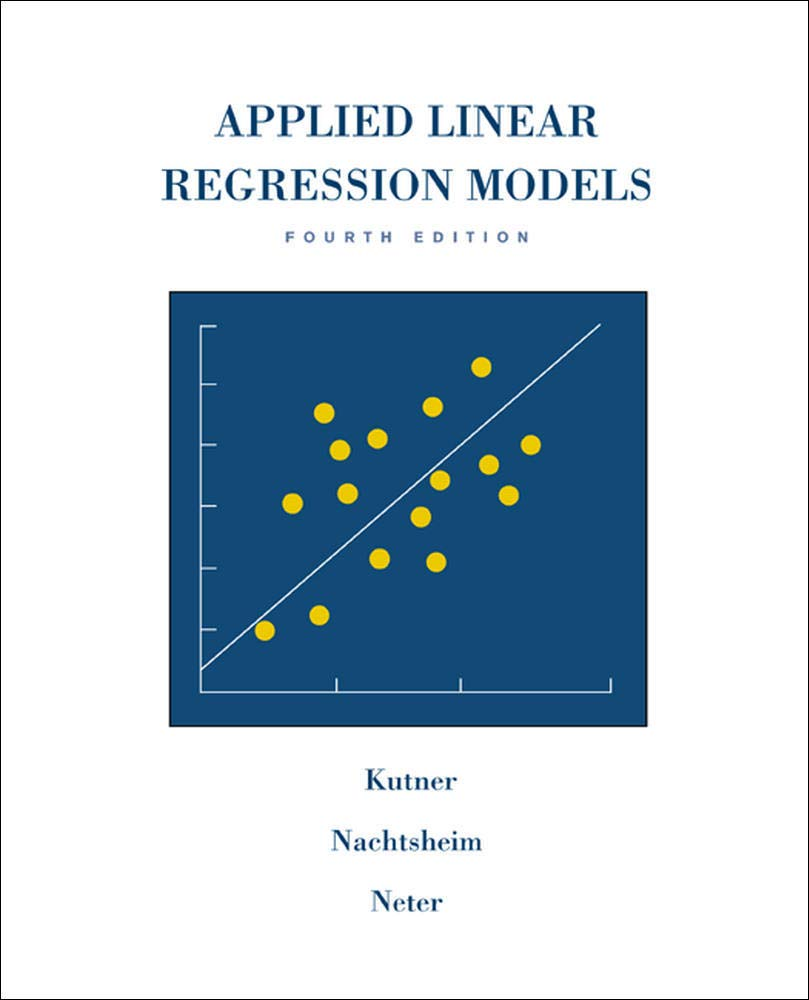
\includegraphics[height=.7\textheight]{figures/AppliedLinearRegressionBook.png}
        
        \vspace{1.5pt}

        \footnotesize

        Applied Linear Regression Models- 4th Edition (McGraw Hill/Kutner, Michael,Nachtsheim, Christopher,Neter, John)

    \end{center}
        \end{columns}
        
    \end{frame}

%------------------------------------------------
\begin{frame}{Setting up the Linear Regression Problem}
    
\begin{center}
    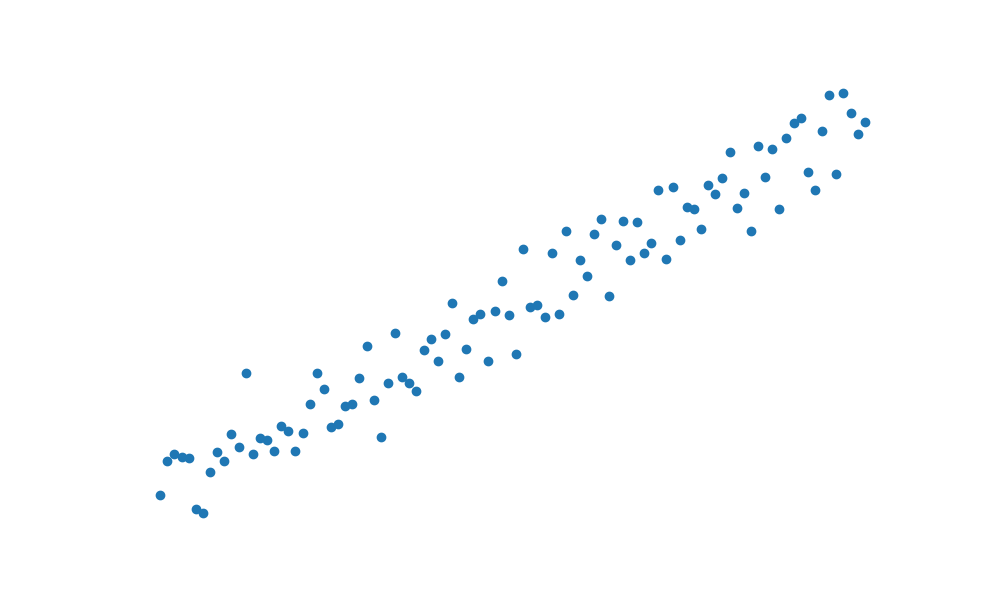
\includegraphics[width=0.7\linewidth]{figures/scatterplot.png}

    What kind of relationship we see here?
\end{center}

\end{frame}

%------------------------------------------------
\begin{frame}{Setting up the Linear Regression Problem}
    
    \begin{center}
        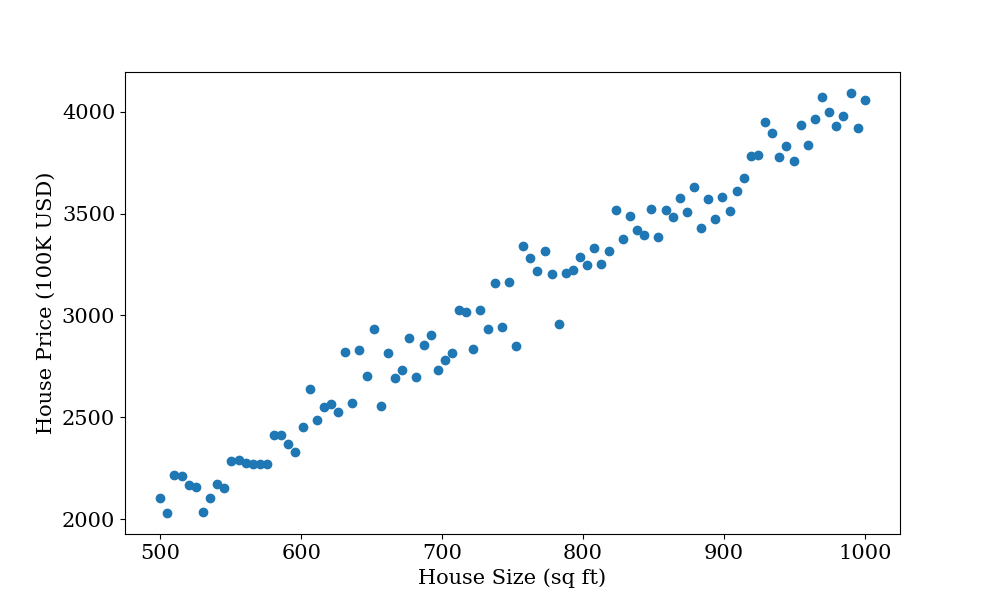
\includegraphics[width=0.7\linewidth]{figures/scatterplot_2.png}
    
        Can we guess the price of house for a size of 650 sq ft?
    \end{center}
    
    \end{frame}
    
    %------------------------------------------------
\begin{frame}{Setting up the Linear Regression Problem}
    
    \begin{center}
        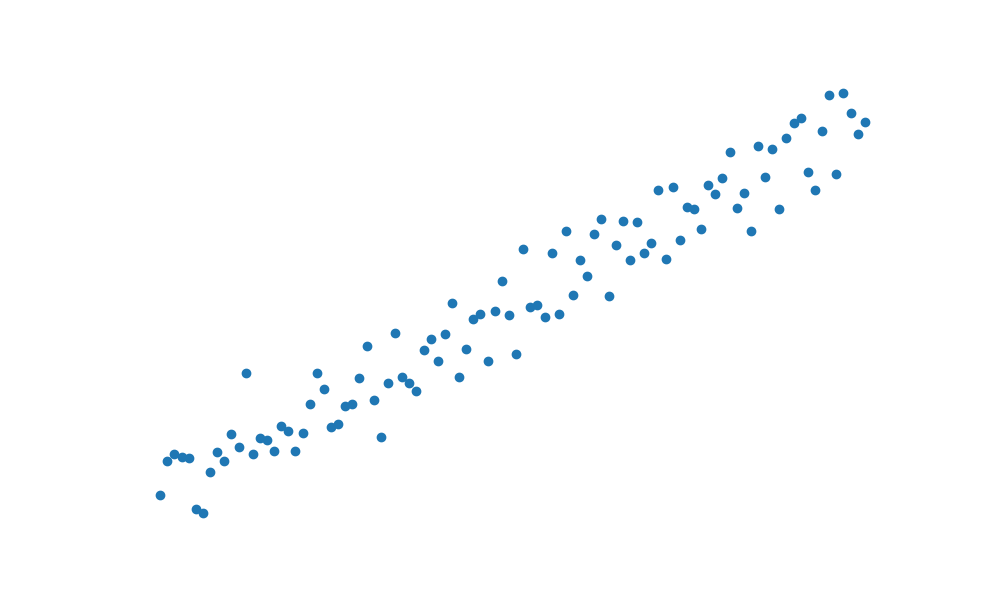
\includegraphics[width=0.7\linewidth]{figures/scatterplot.png}
    
        Can we only fit a straight line?
    \end{center}
    
    \end{frame}




%------------------------------------------------
\begin{frame}{Setting up the Linear Regression Problem}
    \begin{tblock}{Definition}
        Linear regression is a kind of supervised machine learning algorithm where a linear discriminant model $g(\xbf)$  (a straight line) is used to fit on the given dataset. 
    \end{tblock}
    
We define a linear model as $g(\x) = \wbf^\T \x + w_0$.


\end{frame}


%------------------------------------------------

\begin{frame}{Simple Linear Regression/SLR (One Predictor Variable)}
    For simplicity, we first consider a one-dimensional feature vector and one-dimensional label.
\end{frame}


\begin{frame}[containsverbatim]{SLR in Python Using Scikit-Learn}

    \begin{tblock}{Reading Data}

        \begin{minted}
            [
            framesep=1mm,
            baselinestretch=1.2,
            fontsize=\footnotesize
            ]
            {python}
import numpy as np
import matplotlib.pyplot as plt
import pandas as pd
from sklearn.linear_model import LinearRegression, Ridge, Lasso
from sklearn.model_selection import train_test_split, cross_val_score
from statistics import mean

# Read data
data = pd.read_csv("../Data/HousePrices/kc_house_data.csv")
data.dropna(inplace=True) #remove drop na (not a number)
data.head()
        \end{minted}

    \end{tblock}
    
\end{frame}

\begin{frame}[containsverbatim]{SLR in Python Using Scikit-Learn}

    \begin{center}
        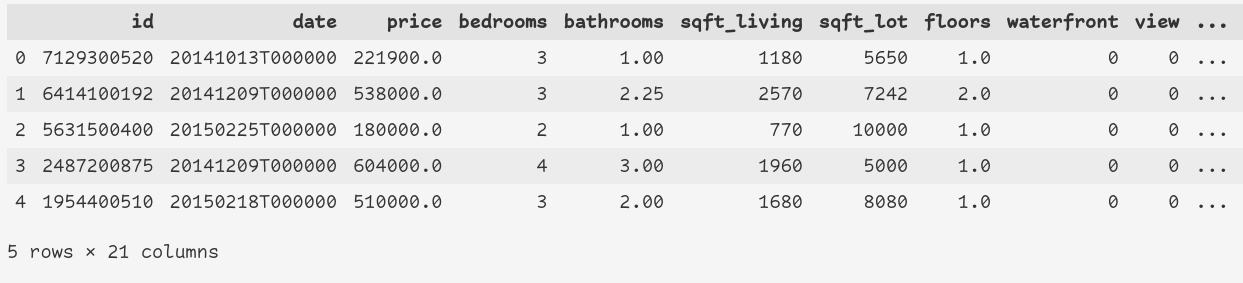
\includegraphics[width=0.99\linewidth]{figures/house_dataframe.png}
    \end{center}
    
\end{frame}


\begin{frame}[containsverbatim]{SLR in Python Using Scikit-Learn}

    \begin{tblock}{Get the independent (explanatory or predictor) and dependent (response) variable}

        \begin{minted}
            [
            framesep=1mm,
            baselinestretch=1.2,
            fontsize=\footnotesize
            ]
            {python}
y = data['price']
X = data[['sqft_living']]          
        \end{minted}
    \end{tblock}
    Ensure X is a 2D array because scikit-learn Linear Regressione expects 2D Array (n\_samples, n\_features)).  Even if there is only one feature, it still needs to be shaped as a 2D array with one column.
    
\end{frame}

\begin{frame}[containsverbatim]{SLR in Python Using Scikit-Learn}

    \begin{tblock}{Plot between independent and dependent variable}

        \begin{minted}
            [
            framesep=1mm,
            baselinestretch=1.2,
            fontsize=\footnotesize
            ]
            {python}
import seaborn as sns
fig, ax = plt.subplots(figsize=(10, 6))
# We will use seaborn for plotting
sns.scatterplot(x='sqft_living', y='price', data=data, ax=ax)
fig.patch.set_alpha(0.0)
plt.xlabel('House Size (sq ft)')
plt.ylabel('House Price')
plt.show()
        \end{minted}
    \end{tblock}    
\end{frame}

\begin{frame}[containsverbatim]{SLR in Python Using Scikit-Learn}

    \begin{center}
        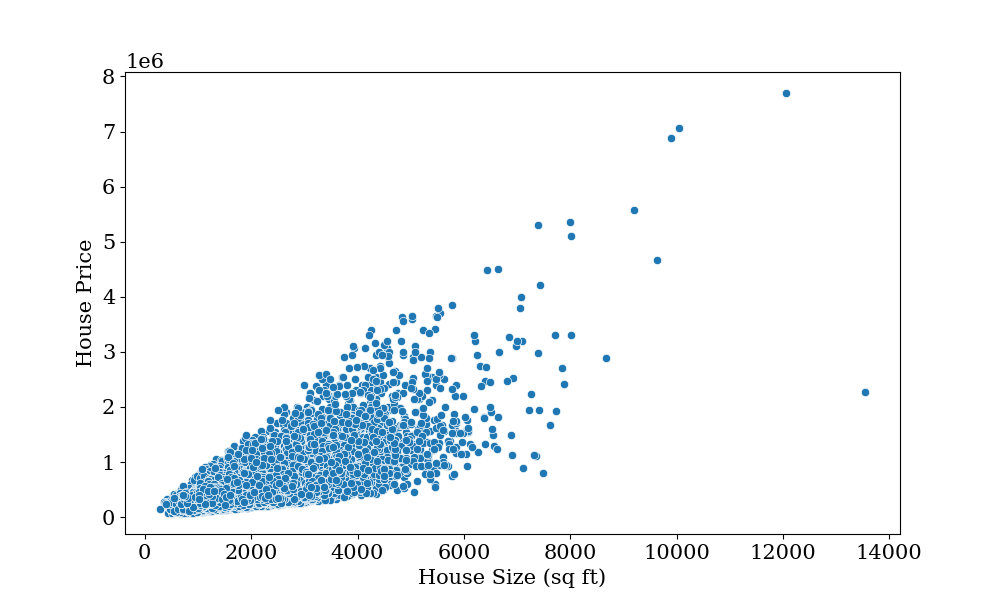
\includegraphics[width=0.75\linewidth]{figures/scatterplot_3.png}
    \end{center}
    
\end{frame}

\begin{frame}[containsverbatim]{SLR in Python Using Scikit-Learn}

    \begin{tblock}{Dividing the data into training and testing set}

        \begin{minted}
            [
            framesep=1mm,
            baselinestretch=1.2,
            fontsize=\footnotesize
            ]
            {python}
X_train, X_test, y_train, y_test = train_test_split(X, y, test_size = 0.25)
        \end{minted}
    \end{tblock}    
    We divide the dataset into training and test data. Test data contains  25\% of the overall data points. Model is being trained using training dataset while model is evaluated using test dataset.
\end{frame}

\begin{frame}[containsverbatim]{SLR in Python Using Scikit-Learn}

    \begin{tblock}{Building the Linear Regression Model using One Feature Only}

        \begin{minted}
            [
            framesep=1mm,
            baselinestretch=1.2,
            fontsize=\footnotesize
            ]
            {python}
linearModel = LinearRegression()
linearModel.fit(X_train, y_train)
 
# Evaluating the Linear Regression model on the test dataset
# coefficient of determination of the prediction
print(linearModel.score(X_test, y_test))
        \end{minted}
    \end{tblock}    
 For this training the evaluation score was 0.46 which is not very good, because relationship between dependent and independent variables are not strongly linear as we saw earlier in the scatter  plot.
\end{frame}

\begin{frame}[containsverbatim]{SLR in Python Using Scikit-Learn}

    \begin{tblock}{Make a Prediction on trained model using a new data point}

        \begin{minted}
            [
            framesep=1mm,
            baselinestretch=1.2,
            fontsize=\footnotesize
            ]
            {python}
new_data_point = pd.DataFrame({'sqft_living': [5000]})

# Make the prediction
predicted_price = linearModel.predict(new_data_point)

print(f"Predicted house price with 5000 sqft living area: ${predicted_price[0]:,.2f}")
        \end{minted}
    \end{tblock}    
Output: Predicted house price with 5000 sqft living area: \$1,372,166.50

\end{frame}

%------------------------------------------------
\begin{frame}{Linear Model for SLR}
    \begin{facts}{}
        \begin{equation}
            g(x) = w_0 + w_1 x
        \end{equation}
    \end{facts}
    We will denote $g(x)$ as $\hat{y}$ from now onwards as it is \textbf{predicted} value. $w_1$ is the slope, and $w_0$ is the y-intercept.
\end{frame}

%------------------------------------------------
\begin{frame}{Data Model and Assumptions for SLR}
    As input data is $\Dcal:=\{(\x_i, y_i)\}_{i=1}^n$, we imagine that the actual equation that models the physical process may be 
    \begin{equation}
        y_i = (w_0 + w_1 x_i) + \epsilon_i
    \end{equation}
    which in essence says that $ Y = signal + noise$. $\epsilon_i$ is the random error or noise term.

\begin{gradblock}
        \textbf{For simplicity, we assume that the noise is zero-mean, constant variance noise.}
    \begin{itemize}
        \item $\Ebb[\epsilon_i] = 0 ~\forall~ i$.
        \item $\sigma^2[\epsilon_i] = \sigma^2$ ( a constant) $\forall~ i$.
        \item $\sigma[\epsilon_i, \epsilon_j] = 0~\forall~ i\neq j$.
    \end{itemize}
\end{gradblock}
\end{frame}

%------------------------------------------------
\begin{frame}{Validity of Model and Our Assumption}
    We see that 
    \begin{equation}
        \begin{aligned}
            \Ebb[y_i] & = \Ebb[w_0 + w_1x_i + \epsilon_i] = \Ebb[w_0 + w_1x_i] + \Ebb[\epsilon_i]\\
            & = w_0 + w_1x_i + \Ebb[\epsilon_i]
            & = w_0 + w_1x_i 
        \end{aligned}
    \end{equation}
    This was possible as $w_0 + w_1x_i $ is nonrandom, and we consider zero mean Gaussian error. $\Ebb[y_i] = w_0 + w_1x_i$ called mean response.

    Also, 
    \begin{equation}
        \sigma^2[y_i] = \sigma^2[w_0 + w_1x_i + \epsilon_i] = \sigma^2[\epsilon_i] = \sigma^2
    \end{equation}
    as $w_0 + w_1x_i $ is nonrandom.

    We will still see $\sigma[y_i, y_j] = 0 $ for all $i\neq j$.
\end{frame}

%------------------------------------------------
\begin{frame}{Regression and Least Square}
    \begin{enumerate}
        \item The problem of regression becomes finding $w_0$ and $w_1$.
        \item We use \textbf{Least Square} method to estimate $w_0$, and $w_1$. We will denote estimated $\what_0$, and $\what_1$.
        \item The fitted value would be $\yhat_i = \what_0 + \what_1 x_i$.
    \begin{facts}{}
        We want to minimize {\Huge\begin{equation*}
            Q = \sum(y_i - \yhat_i)^2.
        \end{equation*}
        }
    \end{facts}
    \item Residuals are $e_i = y_i - \yhat_i$. We want residuals to be as low as possible.
    \end{enumerate}
    \end{frame}


    %------------------------------------------------
\begin{frame}{Regression Line and Residuals}
    % \begin{center}
    %     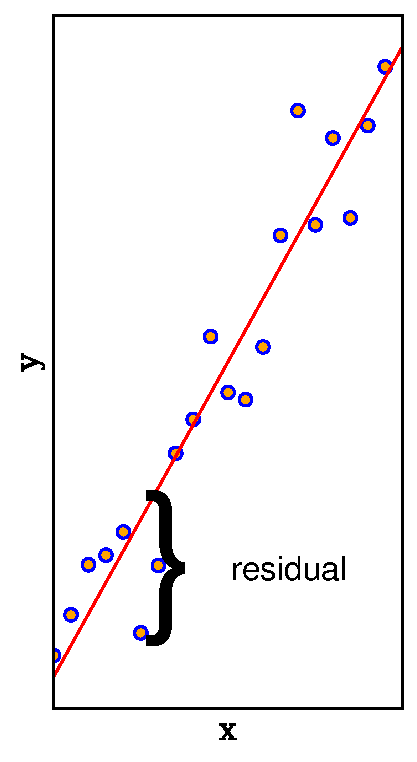
\includegraphics[height=0.75\textheight]{figures/regression_line.pdf}
    % \end{center}
    \begin{columns}
    \column{.3\textwidth}
    
    \begin{center}
    \begin{overpic}[height=0.8\textheight,unit=1pt]{figures/regression_line.pdf}
        \put (35,50) {\textbf{residual}}
         \put (30.5,50) {\pmb{\}}}
    \end{overpic}
     \end{center}
    
    \column{.7\textwidth}
    Here, points are data points, and the line is $\what_0 + \what_1 x_i$.
    \end{columns}
\end{frame}

%------------------------------------------------
\begin{frame}{Solving for $w_0$ and $w_1$: Normal Equations}
    We find that the least square estimators solve the following system  of equations:
    \begin{facts}{}
    {\Huge
    \begin{equation*}
        \begin{aligned}
            \sum y_i & = n \what_0 + \what_1\sum x_i\\
            \sum x_i y_i & = \what_0 \sum x_i + \what_1 \sum x_i^2
        \end{aligned}
    \end{equation*}
    }\end{facts}
    They are called \textbf{normal equations} for the least-square estimators.
    \end{frame}


    %------------------------------------------------
\begin{frame}{Gauss-Markov Theorem}
    \begin{center}
       \textbf{ The Gauss-Markov theorem says that, under certain conditions, the ordinary least squares (OLS) estimator of the coefficients of a linear regression model is the best linear unbiased estimator.}
    \end{center}
    The Gauss-Markov theorem tells us that using normal equations, we can get the least square solutions for $\what_0$ and $\what_1$ such they are unbiased and have minimum variance among all unbiased linear estimators, i.e.
    \begin{equation}
        \begin{aligned}
            \Ebb[\what_j] = w_j, \quad j = 0, 1
        \end{aligned}
    \end{equation}
    and $\sigma^2[\what_0$] and $\sigma^2[\what_1]$ are minimized.
    \end{frame}

%------------------------------------------------
\begin{frame}{The Least-Square Solution}
    The solution comes out to be the closed form:
    
    
    \begin{gradblock}{}
    {
    \Huge
    \begin{equation*}
    \begin{aligned}
        \what_1 & = \cfrac{\sum_i(x_i - \xbar)(y_i - \ybar)}{\sum_i (x_i - \xbar)^2}\\
        \what_0 & = \ybar - \what_1 \xbar
        \end{aligned}
    \end{equation*}
    }
    \end{gradblock}
    
    \end{frame}

%------------------------------------------------
\begin{frame}{Example: Linear Regression on Toluca Dataset}
    We will consider the Toluca dataset: \url{https://github.com/rahulbhadani/Datasets/blob/master/Toluca/toluca.txt}

    We have
    \begin{itemize}
        \item $x$ = lot size of refrigerator parts production.
        \item $y$ = hours worked (labor)
    \end{itemize}
    at the Toluca manufacturing company.

    \textbf{We have a dataset, what do we do first?}
    
    \vspace{10pt}
    
    \pause
    \begin{facts}{}
        \Huge
        We plot the data first!
    \end{facts}
    
\end{frame}





%------------------------------------------------
\begin{frame}[containsverbatim]{Example: Linear Regression on Toluca Dataset}
    Plot the data first

    \begin{columns}[c]
        \column{.60\textwidth}
        \begin{minted}
            [
            framesep=1mm,
            baselinestretch=1.2,
            fontsize=\footnotesize
            ]
    {python}
toluca = pd.read_csv('../Data/toluca.txt', sep='\t')
x = toluca['LotSize'].to_numpy()
y = toluca['WorkHours'].to_numpy()
plt.rcParams['font.family'] = 'Serif'
plt.rcParams['font.size'] = 15
fig, ax = plt.subplots(figsize=(17, 14))
plt.scatter(x, y, c='orange', edgecolors='blue', s=200)
plt.xlim([0, 123])
plt.xlabel('x: Lot Size')
plt.ylabel('y: Work Hours')
    \end{minted}
    \column{.35\textwidth}
        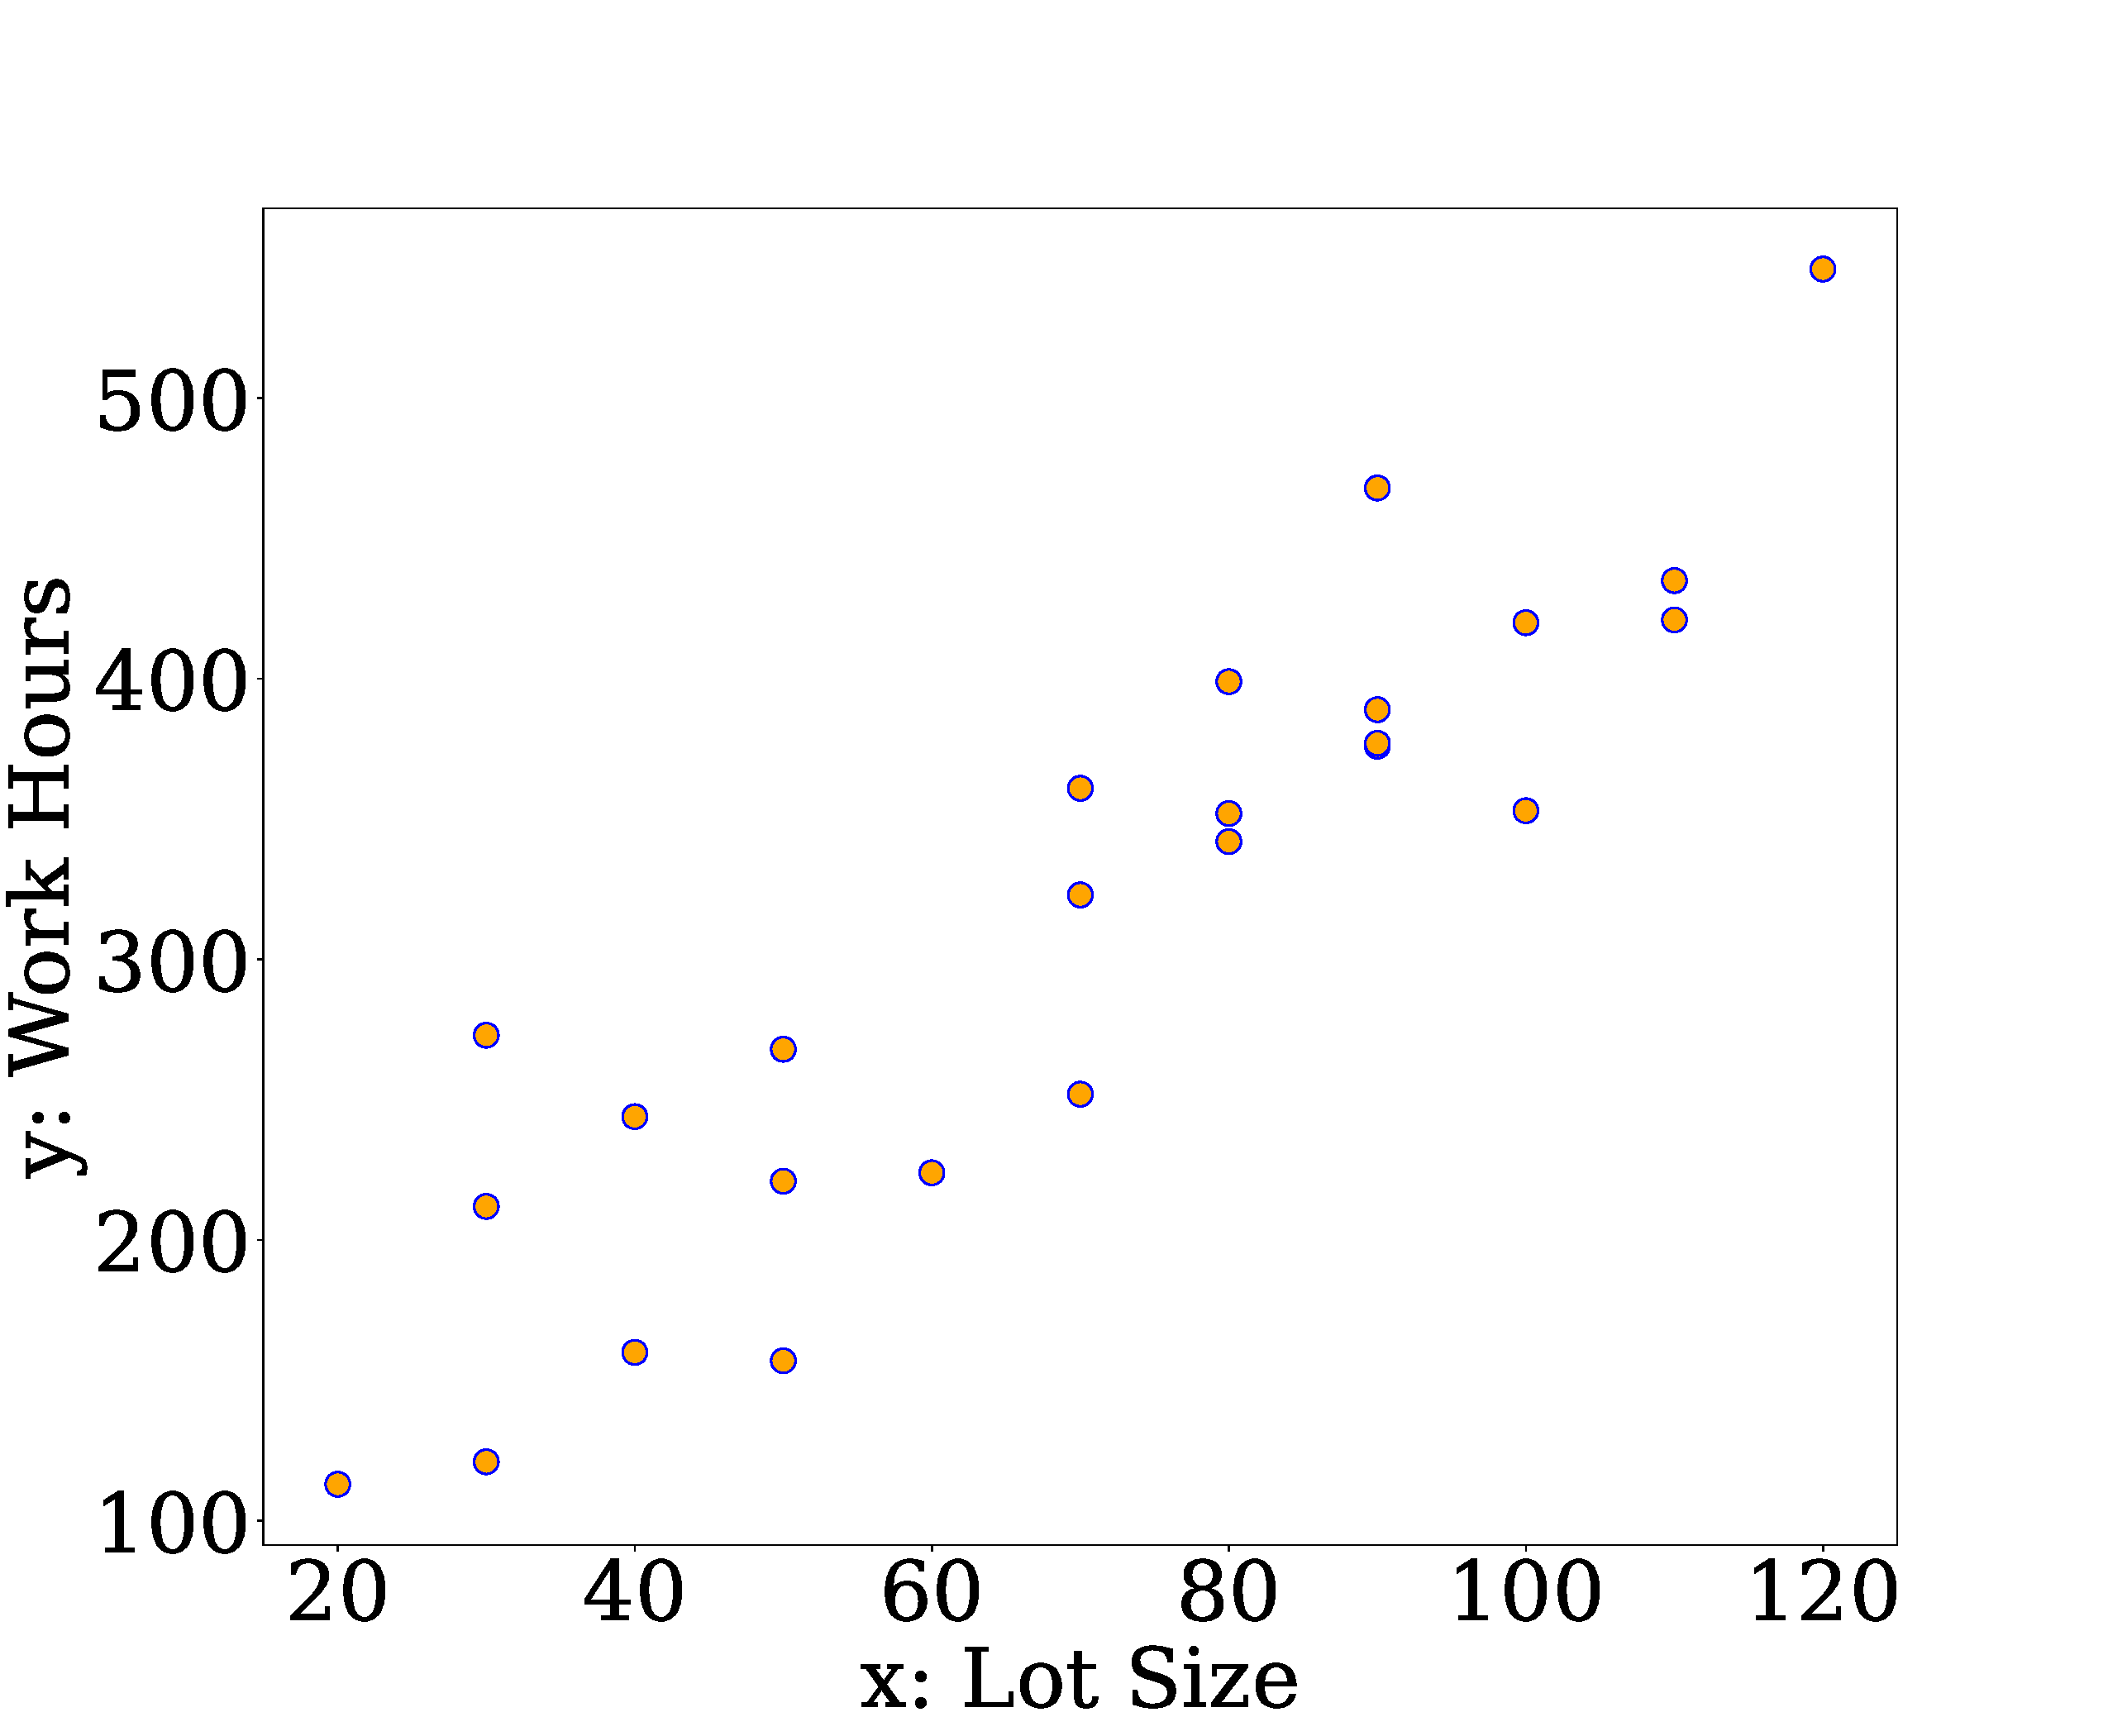
\includegraphics[width=1.0\textwidth]{figures/Toluca_Scatter.pdf}
    \end{columns} 
        \begin{facts}{}
            \large
            We see a linear relationship (sort of!).
        \end{facts}
    \end{frame}


%----------------------------------------------------------------------------------------

%------------------------------------------------
\begin{frame}[containsverbatim]{Example: Linear Regression on Toluca Dataset}
    Fitting the data
    \begin{columns}[c]
        \column{.65\textwidth}
    \begin{minted}
        [
        framesep=1mm,
        baselinestretch=1.2,
        fontsize=\footnotesize
        ]
    {python}
    from sklearn.linear_model import LinearRegression
    reg = LinearRegression().fit(x.reshape((-1, 1)), y)
    print(reg.coef_) # w_1
    print(reg.intercept_) #w_0
    fig, ax = plt.subplots(figsize=(17, 14))
    plt.scatter(x, y, c='orange', edgecolors='blue', s=200)
    plt.xlim([0, 123])
    plt.xlabel('x: Lot Size')
    plt.ylabel('y: Work Hours')
    yhat = reg.coef_*x + reg.intercept_
    plt.plot(x, yhat)
    \end{minted}
    \column{.35\textwidth}
        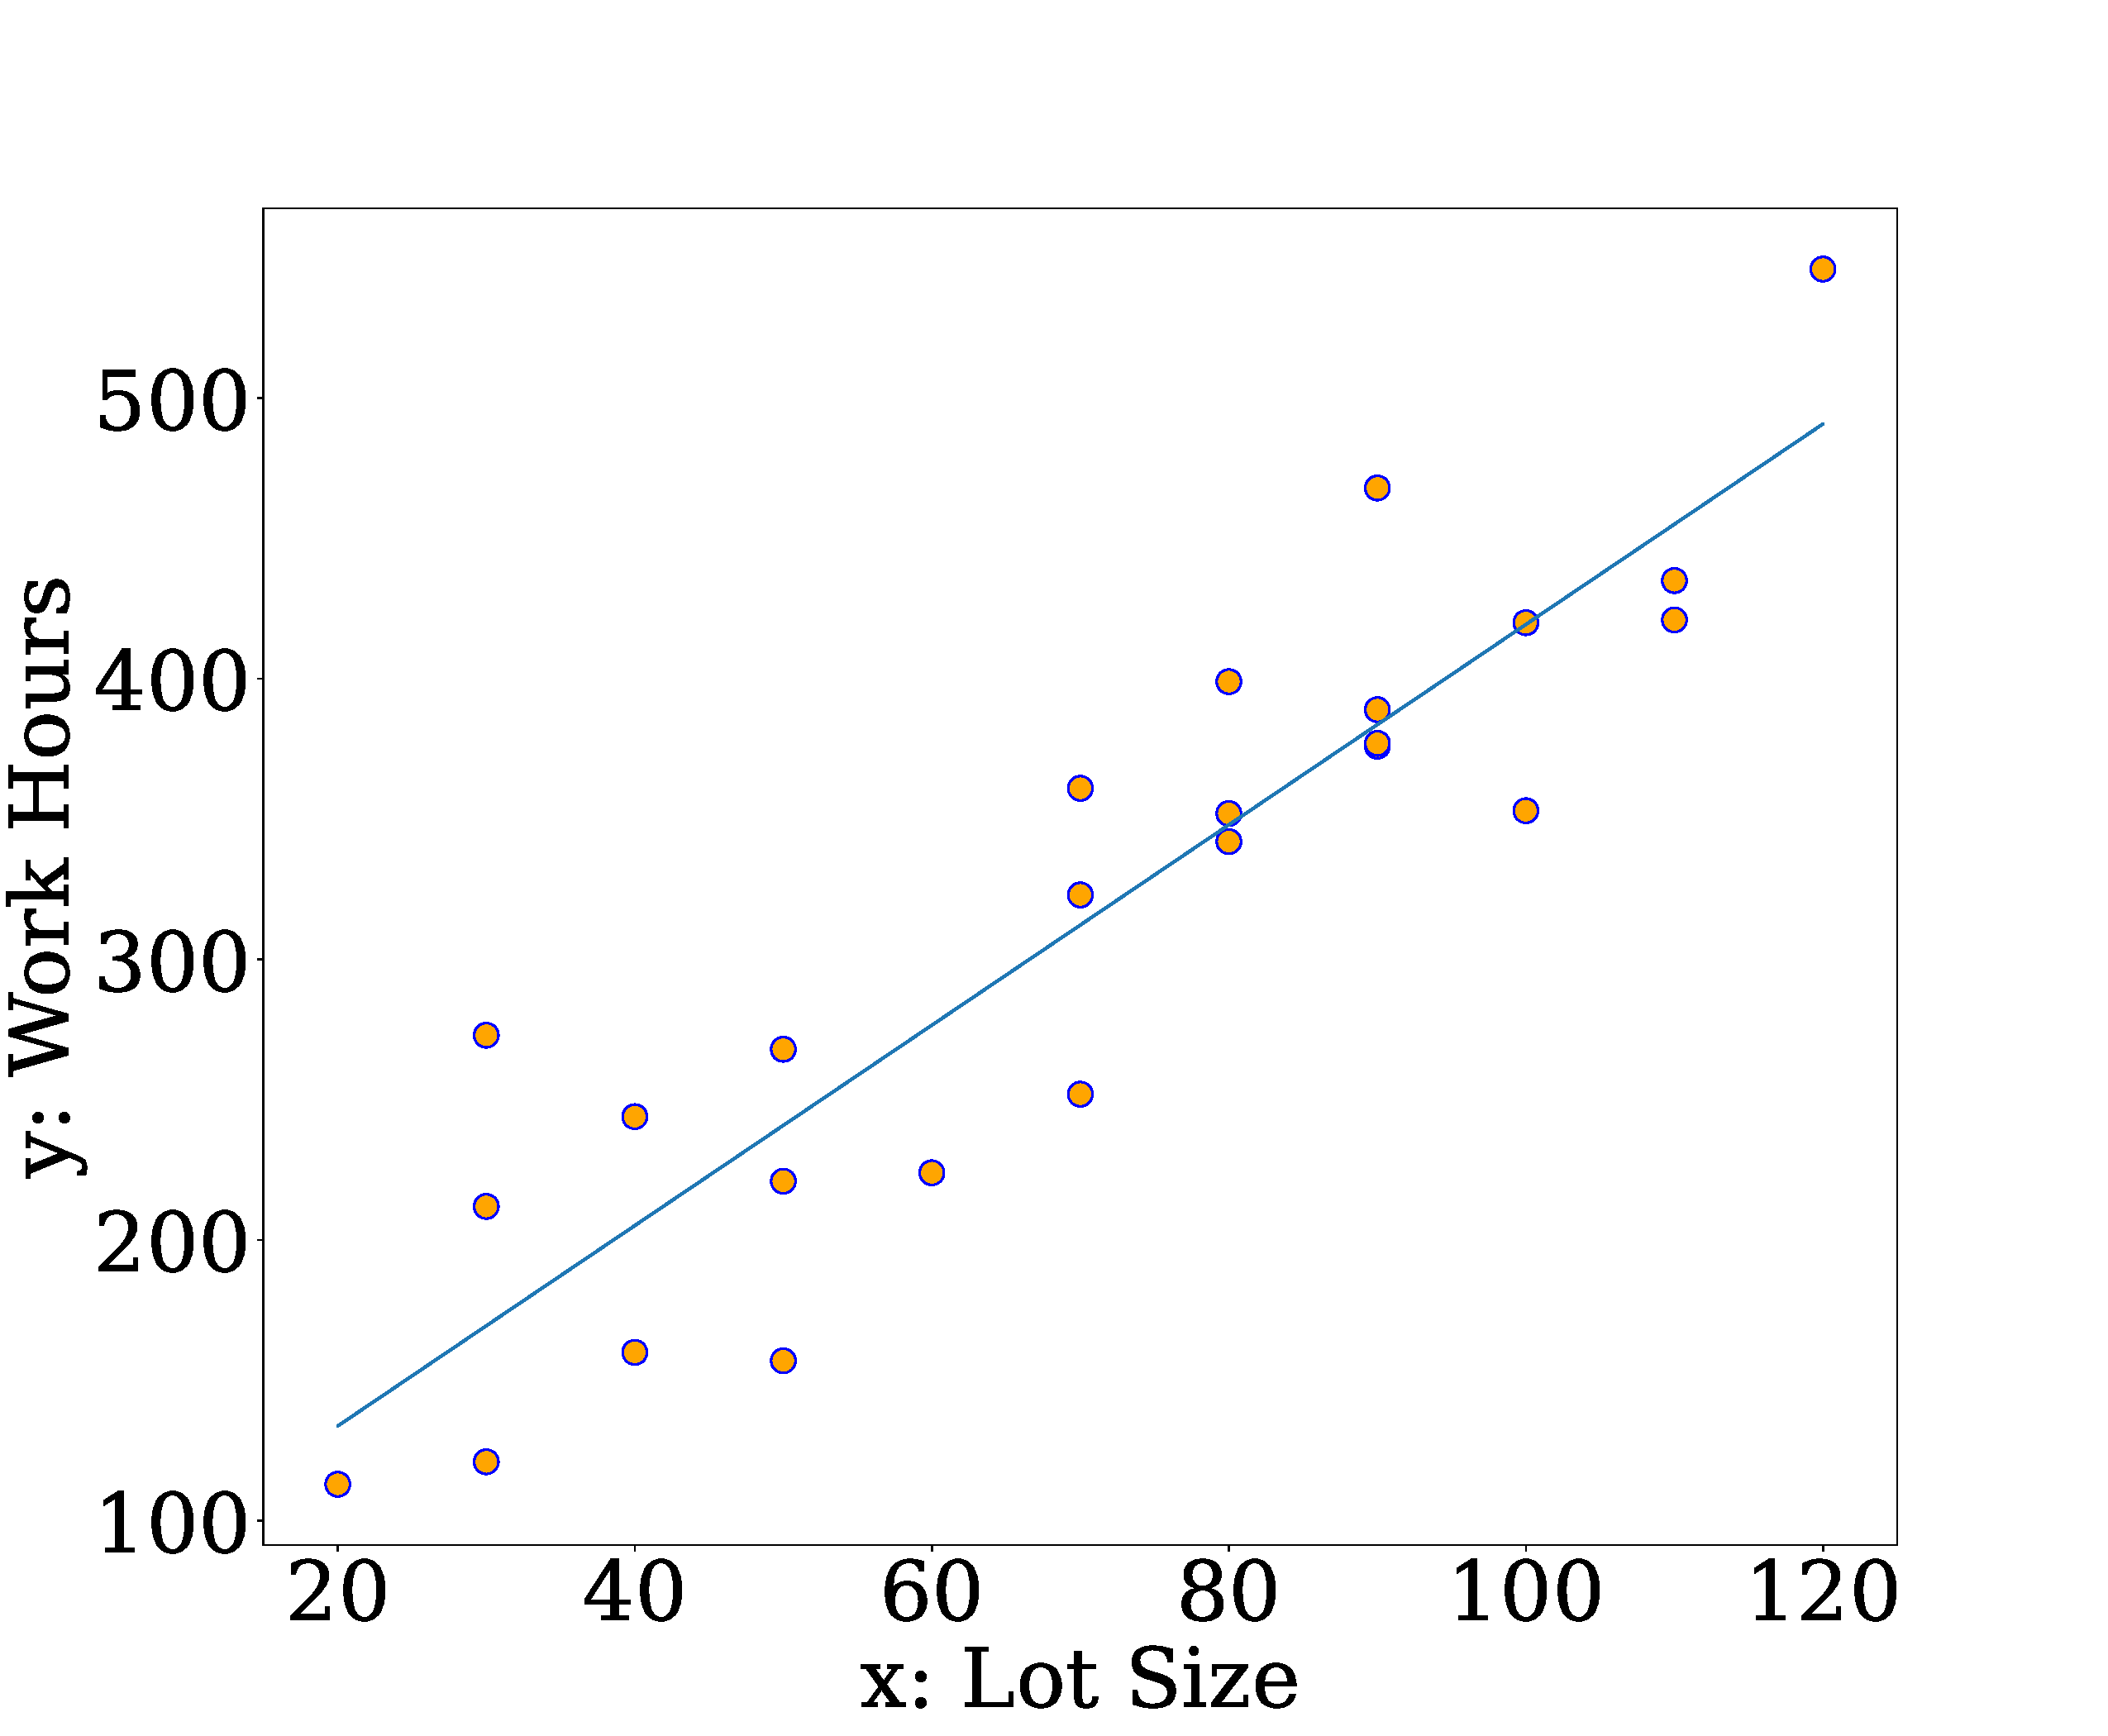
\includegraphics[width=1.0\textwidth]{figures/Toluca_Regressed.pdf}
    \end{columns} 
    \end{frame}
    
    \begin{frame}[containsverbatim]{Prediction on the Fitted Model}
        \begin{minted}
        [
        framesep=1mm,
        baselinestretch=1.2,
        fontsize=\LARGE,
        bgcolor=PapayaWhip,
        ]
        {python}
        reg.predict([[50.0], [100.0]])
        \end{minted}
        Output: array([240.8759596 , 419.38606061])
        \end{frame}
        

        %------------------------------------------------
\begin{frame}{Consequences of the Least-Square Fit}
    We see the following mathematical consequences as a result of the least square fit:
    \begin{enumerate}
        \item  $\sum e_i = 0$.
        \item Sum of squared residuals (errors) $\sum e_i^2$ is minimum.
        \item $\sum y_i = \sum \yhat_i$.
        \item $\sum e_i x_i = 0$ (weighted sum of $e_i$'s is zero).
        \item $\sum e_i \yhat_i = 0$.
        \item $\yhat(\xbar) = \ybar$.
    \end{enumerate}
    \end{frame}
    
    
    %------------------------------------------------
    \begin{frame}{Estimating Variance}
        We want to know how much uncertainty is there in our estimate.
    
    \begin{tblock}{Mean-Squared Error (MSE)}
    \begin{equation}
         \textrm{MSE} = \cfrac{\textrm{SSE}}{\textrm{degree of freedom (df)}} = \cfrac{\sum (y_i -\yhat)^2}{n-2}.
    \end{equation}
    Here the degree of freedom is calculated as \textbf{df = no. of observations - no. of fitted components}.
    
    Mathematically, we can show that $\Ebb[\textrm{MSE}] =\sigma^2$.
    \end{tblock}
    \end{frame}
    
    %------------------------------------------------
    \begin{frame}{Goodness of Fit using Coefficient of Determination $R^2$}
    Goodness of Fit, i.e. how well this linear regression model fits into the given dataset is given by 
    \begin{facts}{}
        {
        \LARGE
        \begin{center}
            \begin{equation*}
        R^2 = 1-\cfrac{\textrm{SSE}}{\textrm{SSTO}}
    \end{equation*}
        \end{center}
        }
    \end{facts}
    
    where $\textrm{SSTO} = \sum (y_i - \ybar)^2$.

    $R^2$ is the percentage of the total variation of the $y_i$ explained by the regression model.

\end{frame}
    
     \begin{frame}{Properties of $R^2$}


    \textbf{Some interesting properties of $R^2$:}
    \begin{enumerate}
        \item $R^2 = 1$ when every point lies on the regression straight line.
        \item $R^2 = 0$ when data are cloudy.
    \end{enumerate}
    \textbf{Some limitations of $R^2$:}
    \begin{enumerate}
        \item $R^2 \to 1$ indicates a strong linear relationship but it might be a poor fit.
        \item $R^2 \to 0$ indicates a weak linear relationship but it may be a good \textbf{nonlinear fit}.
    \end{enumerate}
    
    \end{frame}
    
        %------------------------------------------------

    \begin{frame}[containsverbatim]{Goodness of Fit on Toluca Dataset }
        \begin{minted}
            [
            framesep=1mm,
            baselinestretch=1.2,
            fontsize=\footnotesize
            ]
        {python}
# Calculate and print R^2
r_squared = reg.score(x.reshape((-1, 1)), y)
print("R^2 (Coefficient of Determination):", r_squared)
        \end{minted}
    \end{frame}

    %------------------------------------------------
    \begin{frame}{}
    \Large
    \begin{center}
        Let's pivot a little bit to discuss some concepts needed to build a foundation for additional concepts for linear regression.
    \end{center}
            
    \end{frame}
    %------------------------------------------------
    
    \begin{frame}{Sample Statistics}
        
        \footnotesize

    Consider data points $y_1, y_2, \cdots, y_n$ represent a sample. Then,
    \begin{enumerate}
        \item Sample mean: $\ybar = \cfrac{\sum y_i}{n}$
        \item Sample variance: $s^2 = \cfrac{\sum (y_i - \ybar)^2}{n-1}$
        \item Sample standard deviation: $\sqrt{s^2} = s$.
        \item Degree of freedom: Number of independent elements required to determine some value. (See more: Chapter 2: Design of Experiments, Douglas Montogmery, Page 30, 9th Edition)
        \item For a given normal distribution $Y\sim \Ncal(\mu, \sigma^2)$, then we can create a standard normal random variable by writing $$ Z = \cfrac{Y - \mu }{\sigma}$$.
    \end{enumerate}

    \end{frame}


  %------------------------------------------------
% Frame 1: Introduction to Population and Sample Statistics
%------------------------------------------------
\begin{frame}{Population vs. Sample Statistics}
    \textbf{Population Statistics:}
    \begin{itemize}
        \item Refers to measures computed using the entire population (ideal scenario).
        \item Denoted using Greek letters (e.g., $\mu$, $\sigma^2$).
    \end{itemize}
    \vspace{10pt}
    \textbf{Sample Statistics:}
    \begin{itemize}
        \item Refers to measures computed using a subset (sample) of the population (that's what we know from the data).
        \item Denoted using Latin letters (e.g., $\bar{x}$, $s^2$).
    \end{itemize}
    \end{frame}

    \begin{frame}{Making Inferences (or predictions)}
        \begin{center}
            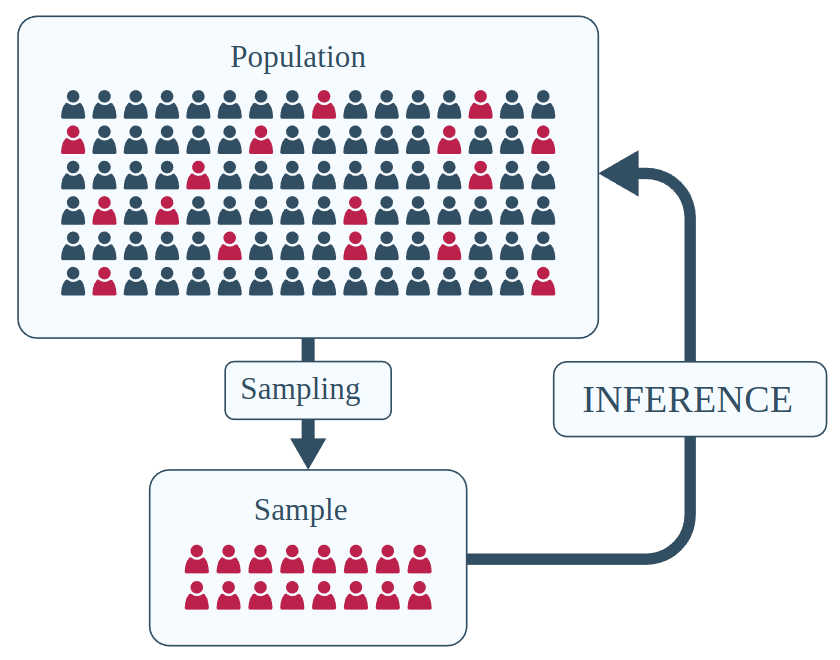
\includegraphics[width=0.4\textwidth]{figures/making_inferences.png}
        \end{center}
        We use data from an observed sample to make a conclusion about a population.


    \end{frame}
    

        %------------------------------------------------

    \begin{frame}{$\chi^2$ Distribution}
        Let $Z_1, Z_2, \cdots, Z_\nu $ be the independent standard random variable. Then we define chi-square ($\chi^2$) random variable as:
        \begin{equation}
            \chi^2(\nu) = Z_1^2 + Z_2^2 + \cdots + Z^2_\nu
        \end{equation}
        where $\nu$ is called the degree of freedom. We have the following results wrt $\chi^2$ distribution:
        \begin{itemize}
            \item $\Ebb[\chi^2(\nu)] = \nu$.
            \item We define $\chi^2(A, \nu)$ as
            $P(\chi^2(\nu)\leq \chi^2(A, \nu) ) = A$. 
           
        \end{itemize}
    
    \end{frame}

    \begin{frame}{Percentile in a Distribution}
        A percentile represents a value below which a certain percentage of observations in a distribution fall.

        Example: The 90th percentile of a distribution means that 90\% of the distribution lies to the left of this value, and 10\% lies to the right.

        Consider that $X$ is a random variable, and we want to know a data point $x$, such that 

        \begin{multiequation}
            P(X \leq x) = 0.90
        \end{multiequation}
        which will gives a value of $x$ such that 90 percent of the data points collected lies to left of $x$ in a PDF graph.

    \end{frame}

    \begin{frame}[containsverbatim]{Percentile in a $\chi^2$ Distribution}

        If $X\sim \chi^2(\nu)$, the 90th percentile of the $\chi^2$ distribution with $\nu = 5$ degrees of freedom is
    $x = \chi^2(.90; 5)$ that satisfies $P(X \leq x) = 0.90$.

    Using either a table or programmatically, $x=9.24$.

    \begin{minted}
        [
        framesep=1mm,
        baselinestretch=1.2,
        fontsize=\footnotesize
        ]
    {python}
from scipy.stats import chi2
# Given percentile and degrees of freedom
percentile = 0.90
degrees_of_freedom = 5
# Calculate the 90th percentile of the chi-squared distribution
chi2_value = chi2.ppf(percentile, degrees_of_freedom)
print(f"The 90th percentile is: {chi2_value:.2f}")
    \end{minted}

    \end{frame}

    %------------------------------------------------

\begin{frame}{PDF of $\chi^2$ Distribution}

        The probability density functions for $\chi^2$ distribution is 
        \begin{equation}
            f(x) = \cfrac{1}{2^{\nu/2}\Gamma(\nu/2)}x^{(\nu/2) - 1}e^{-x/2}, \quad x > 0
        \end{equation}
    
            If $y_1, y_2, \cdots, y_n$ are random samples drawn from $\Ncal(\mu, \sigma^2)$, then 
            \begin{equation}
                \cfrac{\sum (y_i - \ybar)^2}{\sigma^2} \sim \chi^2(n-1)
            \end{equation}
    \textbf{{\color{red}{Note: Some books write $\chi^2_\nu$ instead of $\chi^2(\nu)$.}}}
    
\end{frame}

%------------------------------------------------

\begin{frame}{$\chi^2$ Distribution}

    \begin{center}
    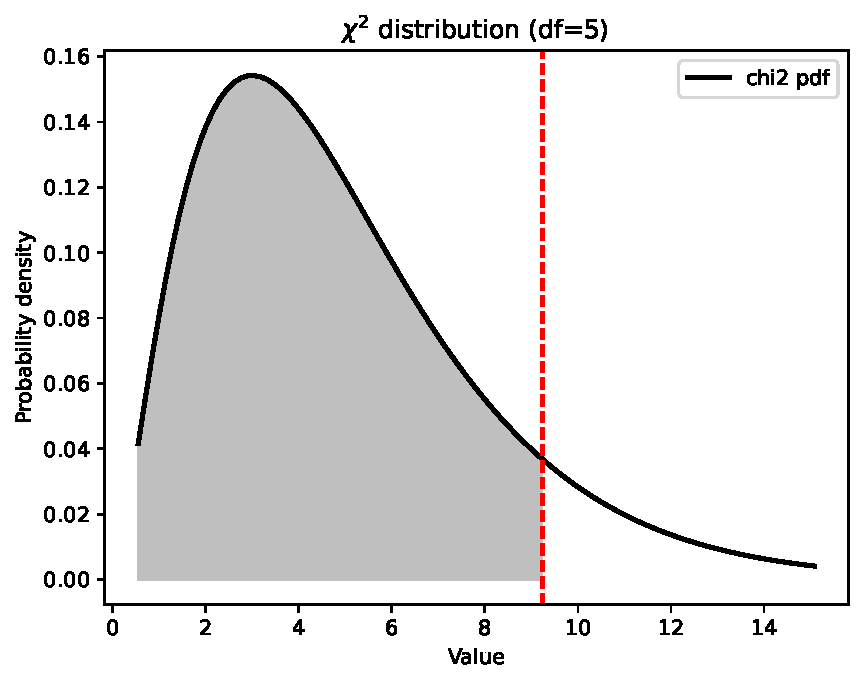
\includegraphics[width=0.50\textwidth]{figures/chi_dist5.pdf}
\end{center}

    \end{frame}
    
    %------------------------------------------------
    \begin{frame}{t Distribution}
    Consider, $Z$, a standard normal random variable, and $\chi^2_\nu$ be another random variable so that they are independent, then
        t distribution, also known as student's t distribution, is written as
        $$
        T_\nu = \cfrac{Z}{\bigg(\chi^2(\nu)/\nu\bigg)^{1/2}}.
        $$

            \end{frame}
    
    %------------------------------------------------
    \begin{frame}{t Distribution}
    
        The PDF of t distribution of $\nu$ degree of freedom is 
        \begin{equation}
            f(t) = \cfrac{\Gamma( \tfrac{\nu+1}{2})}{\sqrt{\nu \pi}\Gamma(\nu/2)} \cfrac{1}{\bigg((t^2/\nu) + 1\bigg) ^{(\nu+1)/2}}, \quad -\infty < t < \infty.
        \end{equation}
    
        If $y_1, y_2, \cdots, y_n$ are random samples drawn from $\Ncal(\mu, \sigma^2)$, then 
        \begin{equation}
            t = \cfrac{\ybar - \mu}{s/\sqrt{n}}
        \end{equation}
        follows the t distribution with $n-1$ degrees of freedom. Here, $s$ is the sample standard deviation.
    \end{frame}
    
    %------------------------------------------------
    \begin{frame}{F Distribution}
    If we have two random variable: $\chi^2_u$ and $\chi^2_v$ with $u$ and $v$ degrees of freedom respectively, then 
    \begin{equation}
        F_{u, v} = \cfrac{\chi^2_u/u}{\chi^2_v/v}
    \end{equation}
    follows F distribution with $u$ numerator degree of freedom, and $v$ denominator degree of freedom.

\end{frame}
    
%------------------------------------------------
\begin{frame}{F Distribution}
    
    Consider two independent normal populations of the common variance $\sigma^2$. If $y_1, y_2, \cdots, y_n$ be random samples of $n$ observations drawn from the first population, and $x_1, x_2, \cdots, x_m$ samples of $m$ observations drawn from the second population, and if their sample variances are $s_y^2$ and $s_x^2$ respectively, then
    
    \begin{equation}
        \cfrac{s_y^2}{s_x^2} \sim F_{n-1, m-1}.
    \end{equation}
    
    \end{frame}
    
    
    %------------------------------------------------
    \begin{frame}{Confidence Interval}
    \begin{tblock}{Definition}
    A confidence interval (CI) is the interval that a population parameter falls between a set of values, i.e. what may be the range of the estimated value. This is important, as estimated values are just estimates and there is some uncertainty about it. CI is measuring that uncertainty.
    \end{tblock}

\end{frame}
    
    
%------------------------------------------------
\begin{frame}{Confidence Interval}
    
    Assume that $\theta$ is the parameter, consider two statistics $\theta_L$ and $\theta_U$ such that
    \begin{equation}
        P(\theta_L \leq \theta \leq \theta_U) = 1-\alpha
    \end{equation}
    is true then the interval $\theta_L \leq \theta \leq \theta_U$ is called a $100(1-\alpha)$ percent confidence interval for the parameter $\theta$. $1 - \alpha$ is called confidence coefficient.
    
    You can understand CI this way:  in repeated random samplings, a large number of such intervals are constructed, and $100(1-\alpha)$ percent of them will contain
    the true value of $\theta$.
    \end{frame}
    

       %------------------------------------------------
       \begin{frame}{}
        \Large
        \begin{center}
            Let's come back to SLR.
        \end{center}
                
        \end{frame}
    
    %------------------------------------------------
% Frame 1: Introduction to SLR Coefficients
%------------------------------------------------
\begin{frame}{Confidence Interval on SLR Coefficients}
    As coefficients (called weights in some literature) $\what_0$ and $\what_1$ are estimates, they have some uncertainty.
    
    We first look at the sampling distribution of $\what_1$.
    
    \begin{gradblock}{}
       \textbf{The sampling distribution of $\what_1$ means that different values of  $\what_1$ would be obtained
    with repeated sampling when the levels of the predictor variable $x$ are held constant from sample to sample.}
    
    \hfill -- Applied Linear Regression Models, \textit{Kutner, Nachtsheim, Neter}
    \end{gradblock}
    \end{frame}
    
    %------------------------------------------------
    % Frame 2: Expectations and Variance of \what_1
    %------------------------------------------------
    \begin{frame}{Expectations and Variance of $\what_1$}
    Expectations and variance of $\what_1$ are
    \begin{equation}
    \begin{aligned}
        \Ebb[\what_1] & = w_1\\
        \sigma^2[\what_1] & = \cfrac{\sigma^2}{\sum (x_i - \xbar)^2}
    \end{aligned}
    \end{equation}
    where $\sigma^2$ is the assumed error variance.
    \end{frame}
    
    %------------------------------------------------
    % Frame 3: Sample Variance for \what_1
    %------------------------------------------------
    \begin{frame}{Sample Variance for $\what_1$}
    Of course, we won't know the $\sigma^2$ because that's a mathematical assumption, so we replace it with $\textrm{MSE}$ defined earlier and hence we have 
    
    \begin{equation}
        s^2[\what_1] = \cfrac{\textrm{MSE}}{\sum (x_i - \xbar)^2}
    \end{equation}
    \end{frame}
    
    %------------------------------------------------
    % Frame 4: The t Distribution
    %------------------------------------------------
    \begin{frame}{The t Distribution}
    In that case, we can follow one statistical theorem that says
    
    \begin{gradblock}{}
         When a statistic is standardized but the denominator is an estimated standard deviation (or variance) rather than the true standard deviation (or variance), then the statistic follows \textbf{t distribution}.
    \end{gradblock}
    
    Thus, 
    \begin{equation}
        T = \cfrac{\what_1 - w_1}{s[\what_1]}
    \end{equation}
    follows a t distribution with $n-2$ degrees of freedom, i.e. $T\sim t_{n-2}$.
    \end{frame}
    
    %------------------------------------------------
    % Frame 5: Confidence Interval for \what_1
    %------------------------------------------------
    \begin{frame}{Confidence Interval for $\what_1$}
    We can write $(1-\alpha)$ CI for $\what_1$ as
    \begin{equation}
    \begin{aligned}
        1 - \alpha & = P \bigg( t(\alpha/2, n - 2) < T < t(1- \alpha/2, n - 2) \bigg)\\
        & = P \bigg( t(\alpha/2, n - 2) <   \cfrac{\what_1 - w_1}{s[\what_1]}< t(1- \alpha/2, n - 2) \bigg)
    \end{aligned}
    \end{equation}
    \end{frame}
    
    %------------------------------------------------
    % Frame 6: Final CI Expression for \what_1
    %------------------------------------------------
    \begin{frame}{Final CI Expression for $\what_1$}
    Hence, we can write the following CI for $\what_1$:
    \begin{gradblock}{}
    {\Huge
    \begin{equation}
    {
        \what_1 \pm t(1- \frac{\alpha}{2}, n - 2)\tikzmarknode{b}{s[\what_1 ]}
    }
    \end{equation}
    }
    \end{gradblock}
    \begin{tikzpicture}[overlay, remember picture]
    \fill[color=red!87, opacity = 0.2] (b.north west) -- (b.north east) -- (b.south east) -- (b.south west) -- cycle;
    \node[below of=b, yshift=-0.5cm, text = blue] (note) {this is one number};
    \draw[->,thick, blue] (note) -- (b.south);
    \end{tikzpicture}
    \end{frame}
    
    %------------------------------------------------
    % Frame 7: Variance of \what_0
    %------------------------------------------------
    \begin{frame}{Variance of $\what_0$}
    Similarly, $\what_0$ follows the Normal distribution $\Ncal(w_0, \sigma^2[\what_0])$ where
    
    \begin{equation}
        \sigma^2[\what_0] = \sigma^2 \times \Big( \cfrac{1}{n} + \cfrac{\xbar^2}{\sum (x_i - \xbar)^2} \Big)
    \end{equation}
    
    Of course, we won't know $\sigma^2$ and hence, it is replaced by the MSE and we have the sample variance for $\what_0$ as
    
    \begin{equation}
        s^2[\what_0] = \textrm{MSE} \times \Big( \cfrac{1}{n} + \cfrac{\xbar^2}{\sum (x_i - \xbar)^2} \Big)
    \end{equation}
    \end{frame}
    
    %------------------------------------------------
    % Frame 8: Confidence Interval for \what_0
    %------------------------------------------------
    \begin{frame}{Confidence Interval for $\what_0$}
    Similar to $\what_1$, the CI for $\what_0$ is
    \begin{gradblock}{}
    {\Huge
    \begin{equation}
    {
        \what_0 \pm t(1- \frac{\alpha}{2}, n - 2)\tikzmarknode{b}{s[\what_0 ]}
    }
    \end{equation}
    }
    \end{gradblock}
    \end{frame}
    
    % %------------------------------------------------
    % \begin{frame}{Confidence Interval on SLR Coefficients}
    % As coefficients (called weights in some literature) $\what_0$ and $\what_1$ are estimates, they have some uncertainty.
    
    % We first look at the sampling distribution of $\what_1$.
    
    % \begin{gradblock}{}
    %    \textbf{The sampling distribution of $\what_1$ means that different values of  $\what_1$ would be obtained
    % with repeated sampling when the levels of the predictor variable $x$ are held constant from sample to sample.}
    
    % \hfill -- Applied Linear Regression Models, \textit{Kutner, Nachtsheim, Neter}
    % \end{gradblock}

    % Expectations and variance of $\what_1$ are
    % \begin{equation}
    % \begin{aligned}
    %     \Ebb[\what_1] & = w_1\\
    %     \sigma^2[\what_1] & = \cfrac{\sigma^2}{\sum (x_i - \xbar)^2}
    % \end{aligned}
    % \end{equation}
    % where $\sigma^2$ is the assumed error variance.
    
    % Of course, we won't know the $\sigma^2$ because that's a mathematical assumption, so we replace it with $\textrm{MSE}$ defined earlier and hence we have 
    
    % \begin{equation}
    %     s^2[\what_1] = \cfrac{\textrm{MSE}}{\sum (x_i - \xbar)^2}
    % \end{equation}
    
    % In that case, we can follow one statistical theorem that says
    
    % \begin{gradblock}{}
    %      When a statistic is standardized but the denominator is an estimated standard deviation (or variance) rather than the true standard deviation (or variance), then the statistic follows \textbf{t distribution}.
    % \end{gradblock}
    
    % Thus, 
    % \begin{equation}
    %     T = \cfrac{\what_1 - w_1}{s[\what_1]}
    % \end{equation}
    % follows a t distribution with $n-2$ degrees of freedom, i.e. $T\sim t_{n-2}$.
    
    % We can write $(1-\alpha)$ CI for $\what_1$ is based on as 
    % \begin{equation}
    % \begin{aligned}
    %     1 - \alpha & = P \bigg( t(\alpha/2, n - 2) < T < t(1- \alpha/2, n - 2) \bigg)\\
    %     & = P \bigg( t(\alpha/2, n - 2) <   \cfrac{\what_1 - w_1}{s[\what_1]}< t(1- \alpha/2, n - 2) \bigg)\
    % \end{aligned}
    % \end{equation}
    
    % \newpage
    % Hence, we can write the following CI for $\what_1$:
    % \begin{gradblock}{}
    % {\Huge
    % \begin{equation}
    % {
    %     \what_1 \pm t(1- \frac{\alpha}{2}, n - 2)\tikzmarknode{b}{s[\what_1 ]}
    % }
    % \end{equation}
    % }
    % \end{gradblock}
    % \begin{tikzpicture}[overlay, remember picture]
    % \fill[color=red!87, opacity = 0.2] (b.north west) -- (b.north east) -- (b.south east) -- (b.south west) -- cycle;
    % \node[below of=b, yshift=-0.5cm, text = blue] (note) {this is one number};
    % \draw[->,thick, blue] (note) -- (b.south);
    % \end{tikzpicture}
    
    % Similarly, $\what_0$ follows the Normal distribution $\Ncal(w_0, \sigma^2[\what_0]$ where
    
    % \begin{equation}
    %     \sigma^2[\what_0] = \sigma^2\Big( \cfrac{1}{n} + \cfrac{\xbar^2}{\sum (x_i - \xbar)^2} \Big)
    % \end{equation}
    
    % Of course, we won't know $\sigma^2$ and hence, it is replaced by the MSE and we have the sample variance for $\what_0$ as
    
    % \begin{equation}
    %     s^2[\what_0] = \textrm{MSE}\Big( \cfrac{1}{n} + \cfrac{\xbar^2}{\sum (x_i - \xbar)^2} \Big)
    % \end{equation}
    
    
    % and similar to $\what_1$, the CI for $\what_0$ is
    
    % \begin{gradblock}{}
    % {\Huge
    % \begin{equation}
    % {
    %     \what_0 \pm t(1- \frac{\alpha}{2}, n - 2)\tikzmarknode{b}{s[\what_0 ]}
    % }
    % \end{equation}
    % }
    % \end{gradblock}
    % \end{frame}
    
    % %------------------------------------------------
    % \begin{frame}{Making Inference and CI on a new Predictor}
    %     Assume that we want to make a prediction at a new predictor $x_h$.
    
    %     \begin{itemize}
    %         \item The least square estimator will give $\yhat_h = \what_0 + \what_1 x_h$.
    %     \end{itemize}
    
    % We find that the expectations and the sample variance of $\yhat_h$ are
    % \begin{equation}
    %     \begin{aligned}
    %         \Ebb[\yhat_h] & = w_0 + w_1 x_h\\
    %         s^2[\yhat_h] & = \textrm{MSE}\bigg( \cfrac{1}{n} + \cfrac{(x_h - \xbar)^2}{\sum (x_i - \xbar)^2} \bigg)
    %     \end{aligned}
    % \end{equation}
    
    % \newpage
    % Fortunately, we won't need to know the exact $w_0$ and $w_1$ to construct the CI for $y_h$. It will just be 
    
    % \begin{gradblock}{}
    % {\Huge
    % \begin{equation}
    % {
    %     \yhat_h \pm t(1- \frac{\alpha}{2}, n - 2)\tikzmarknode{b}{s[\yhat_h ]}
    % }
    % \end{equation}
    % }
    % \end{gradblock}
    
    % \newpage
    % \textbf{Note:}
    % The above CI is based on the assumption that $x_h$ comes from the same trial as the original data. If $x_h$ is obtained from another experiment, that is independent of the data used to develop the regression model, we may need to account for additional prediction error $\epsilon_h$, which still has the same variance $\sigma^2$. In such a case, the sample variance will be 
    
    % $$
    % \textrm{MSE}\bigg( 1+ \cfrac{1}{n} + \cfrac{(x_h - \xbar)^2}{\sum (x_i - \xbar)^2} \bigg).
    % $$
    % Refer to Section 2.4 and 2.5 of \textbf{Applied Linear
    % Regression Models, \textit{Kutner, Nachtsheim, and Neter}, 4th Ed.}
    % \end{frame}
    
    %------------------------------------------------
% Frame 1: Prediction at a New Predictor
%------------------------------------------------
\begin{frame}{Making Inference and CI on a New Predictor}
    Assume that we want to make a prediction at a new predictor $x_h$.
    
    \begin{itemize}
        \item The least square estimator will give $\yhat_h = \what_0 + \what_1 x_h$.
    \end{itemize}
    
    We find that the expectations and the sample variance of $\yhat_h$ are
    \begin{equation}
        \begin{aligned}
            \Ebb[\yhat_h] & = w_0 + w_1 x_h\\
            s^2[\yhat_h] & = \textrm{MSE} \times \bigg( \cfrac{1}{n} + \cfrac{(x_h - \xbar)^2}{\sum (x_i - \xbar)^2} \bigg)
        \end{aligned}
    \end{equation}
    \end{frame}
    
    %------------------------------------------------
    % Frame 2: Confidence Interval for $\yhat_h$
    %------------------------------------------------
    \begin{frame}{Confidence Interval for $\yhat_h$}
    Fortunately, we won't need to know the exact $w_0$ and $w_1$ to construct the CI for $y_h$. It will just be 
    
    \begin{gradblock}{}
    {\Huge
    \begin{equation}
    {
        \yhat_h \pm t(1- \frac{\alpha}{2}, n - 2)\tikzmarknode{b}{s[\yhat_h ]}
    }
    \end{equation}
    }
    \end{gradblock}
    \end{frame}
    
    %------------------------------------------------
    % Frame 3: Additional Considerations for $x_h$
    %------------------------------------------------
    \begin{frame}{Additional Considerations for $x_h$}
    \textbf{Note:}
    The above CI is based on the assumption that $x_h$ comes from the same trial as the original data. If $x_h$ is obtained from another experiment, that is independent of the data used to develop the regression model, we may need to account for additional prediction error $\epsilon_h$, which still has the same variance $\sigma^2$. In such a case, the sample variance will be 
    
    $$
    \textrm{MSE} \times \bigg( 1+ \cfrac{1}{n} + \cfrac{(x_h - \xbar)^2}{\sum (x_i - \xbar)^2} \bigg).
    $$
    Refer to Section 2.4 and 2.5 of \textbf{Applied Linear Regression Models, \textit{Kutner, Nachtsheim, and Neter}, 4th Ed.}
    \end{frame}

    
    \begin{frame}{Confidence Bands}
    We may also want a confidence band for the entire regression line $\Ebb[Y] = w_0 + w_1 X$.
    
    It is given by Working \& Hotelling (1929) and Scheffe (1953) as:
    \begin{equation}
        \yhat_h \pm W_\alpha s[\yhat]
    \end{equation}
       for any value of $y_h$ where $W_\alpha = \sqrt{2 F(1-\alpha; 2, n-2)}$; $F$ is the F distribution.
    
    \vspace{3em} 
    These bands, called WHS bands are in the shape of parabolas.
    \end{frame}
    
    \begin{frame}{Confidence Band: An Example}

        \begin{center}
            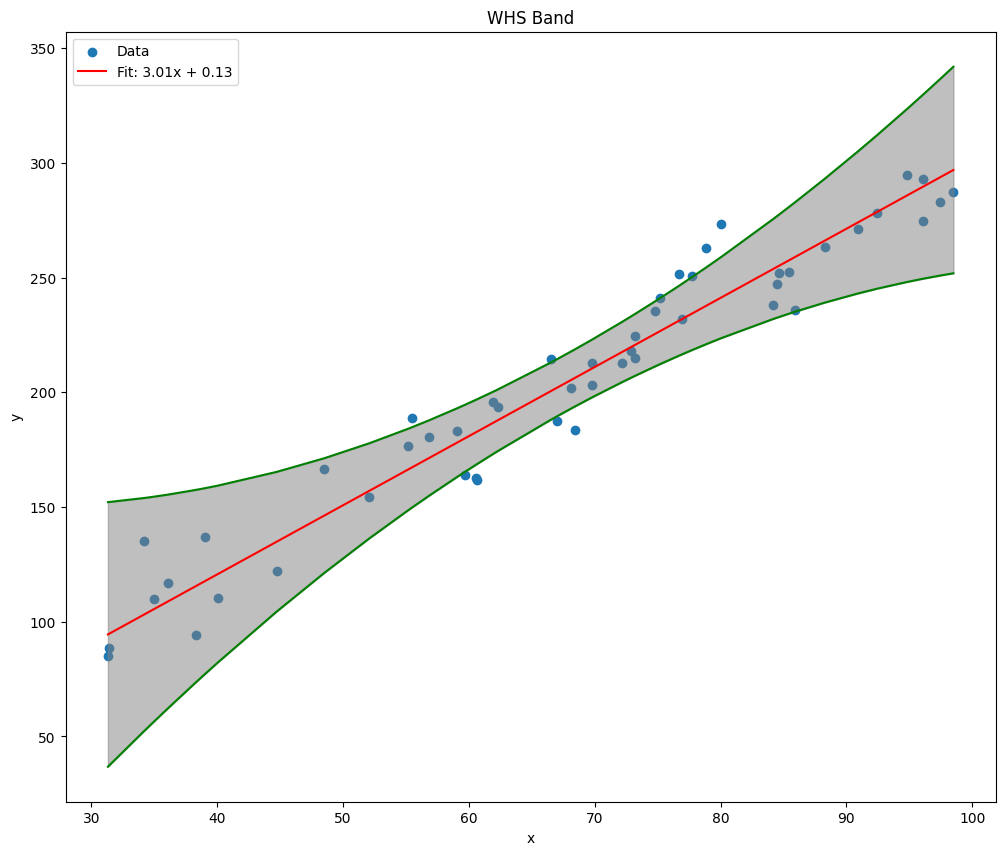
\includegraphics[width=0.5\textwidth]{figures/confidence_band.png}
        \end{center}
        
    \end{frame}
    %%%%%%%%%%%%%%%%%%%%%%%%%%%%%%%%%%%%%%%%%%%%%%%%%%%%%
\begin{sectionframe}{\faSignal}{Multiple Linear Regression using Matrix Approach}
\end{sectionframe}


%------------------------------------------------
\begin{frame}{First-order Model with Two Predictor Variables}


        \begin{equation}
            y_i = w_0 + w_1 x_{i1} + w_2 x_{i2} + \epsilon_i
        \end{equation}
        In this case, our general assumption model, as seen in the single predictor variable will hold true, such as $\Ebb[y_i] = w_0 + w_1 x_{i1} + w_2 x_{i2} $.
    
        \vspace{10pt}
        In addition, the following value holds, as you see by taking the partial derivatives of the model:
        \begin{equation}
            \begin{aligned}
                 \cfrac{\partial \Ebb[Y]}{\partial X_1}  = w_1 \quad \quad
                 \cfrac{\partial \Ebb[Y]}{\partial X_2}  = w_2
            \end{aligned}
        \end{equation}
       

    \end{frame}

    %------------------------------------------------
\begin{frame}{First-order Model with more than Two Predictor Variables}

    Consider a regression model with $p-1$ predictor variable:

    
     \begin{equation}
     \begin{aligned}
            y_i & = w_0 + w_1 x_{i1} + w_2 x_{i2} + \cdots + w_{p-1} x_{i(p-1)} \epsilon_i\\
            & =  w_0 + \sum_{k = 1}^{p-1} w_k x_{ik} + \epsilon_i
             \end{aligned}
        \end{equation}
        If we set $x_{i0} = 1$, then we can write:
        \begin{equation}
     \begin{aligned}
            y_i & =   \sum_{k = 0}^{p-1} w_k x_{ik} + \epsilon_i
             \end{aligned}
        \end{equation}

        
    \end{frame}

    %------------------------------------------------
\begin{frame}{Meaning of Linearity in the Regression Model}

    The linear model implies that the model is linear in its parameters, i.e. it can be expressed as
    $$
    y_i = \sum c_{i0}w_i
    $$
     The model such as 
     $$
     y_i = w_0 \exp(w_1 x_i) + \epsilon_i
     $$
     is not linear because we cannot express it as $ \sum c_{i0}w_i$.
    \end{frame}


%------------------------------------------------
% Frame 1: Matrix Representation of Components
%------------------------------------------------
\begin{frame}[allowframebreaks]{Matrix form of the Linear Regression Model}

    \begin{equation}
        \ybf_{n\times 1} = \begin{bmatrix}
            y_1 \\ y_2 \\ \vdots \\  y_n
        \end{bmatrix}
    \quad \quad
          \xbf_{n\times p} = \begin{bmatrix}
            1 & x_{11} & x_{12} & \cdots & x_{1(p-1)}\\
            1 & x_{21} & x_{22} & \cdots & x_{2(p-1)}\\
            \vdots & \vdots & \vdots & \vdots\\
            1 & x_{n1} & x_{n2} & \cdots & x_{n(p-1)}
        \end{bmatrix}    
    \end{equation}
    
    \begin{equation}
        \wbf_{p\times 1} = \begin{bmatrix}
            w_0 \\ w_1 \\ \vdots \\  w_{p-1}
        \end{bmatrix}
    \quad \quad
        \boldsymbol{\epsilon}_{n\times 1} = \begin{bmatrix}
             \epsilon_1 \\  \epsilon_2 \\ \vdots \\  \epsilon_n
        \end{bmatrix}   
    \end{equation}
    \end{frame}
    
    %------------------------------------------------
    % Frame 2: Linear Regression Model in Matrix Form
    %------------------------------------------------
    \begin{frame}[allowframebreaks]{Linear Regression Model in Matrix Form}
    \vspace{10pt}
    In matrix form, we can write it as
    
    \begin{facts}{}
        {\Huge
    
        \begin{equation}
            \ybf_{n\times 1} = \xbf_{n\times p}\wbf_{p\times 1} + \boldsymbol{\epsilon}_{n\times 1}
        \end{equation}
        }
    \end{facts}
    \end{frame}
    
    %------------------------------------------------
    % Frame 3: Expectation and Variance-Covariance Matrix
    %------------------------------------------------
    \begin{frame}[allowframebreaks]{Expectation and Variance-Covariance Matrix}
    Here, $\Ebb[\boldsymbol{\epsilon}] = 0$, and variance-covariance matrix is
    \begin{equation}
        \sigma^2[\boldsymbol{\epsilon}] =  \begin{bmatrix}
            \sigma^2 & 0 & 0 & \cdots & 0\\
            0 & \sigma^2 & 0 & \cdots & 0\\
            \vdots & \vdots & & \vdots \\
            0 & 0 & \cdots & 0 & \sigma^2
        \end{bmatrix} = \sigma^2\Ibf
    \end{equation}
    
    In this case, instead of random variable $Y$, and $X$, we have random vector $\Ybf$, and $\Xbf$, and $\Ebb[\Ybf] = \Xbf \wbf $.
    \end{frame}
    
    %------------------------------------------------
\begin{frame}{Least Square Estimator/Cost Function for MLR}
    \begin{facts}{Cost Function}
    {
    \LARGE
    \begin{equation}
    \begin{aligned}
        J & = \cfrac{1}{2n}\sum_{i=1}^n ( y_i - \sum_{k=0}^{p-1} w_k x_{ik} )^2\\
        & =  \cfrac{1}{2n}\sum_{i=1}^n ( y_i - \wbf^\top \xbf_i )^2 = \cfrac{1}{2n}(\ybf - \xbf \wbf)^\top(\ybf - \xbf \wbf)
        \end{aligned}
    \end{equation}
    }
    \end{facts}
    \end{frame}
    
%------------------------------------------------
% Frame 1: Introducing the Normal Equation
%------------------------------------------------
\begin{frame}{Normal Equation for MLR}
    \begin{facts}{Normal Equation}
    {
    \Large
    \begin{equation}
       \xbf^\top\xbf \hat{\wbf} = \xbf^\top\ybf
    \end{equation}
    How to solve this for $\wbf$?
    }
    \end{facts}
    \end{frame}
    
    %------------------------------------------------
    % Frame 2: Partial Derivative and Solution Derivation
    %------------------------------------------------
    \begin{frame}{Deriving the Solution}
    \begin{facts}{Normal Equation}
    {
    \Large
    \begin{equation}
        \cfrac{\partial J}{\partial \wbf} = -\cfrac{1}{2n}\xbf^\top(\ybf - \xbf \wbf) = 0 \Rightarrow  -\cfrac{1}{2n}(\xbf^\top\ybf - \xbf^\top\xbf \wbf) = 0
    \end{equation}
    }
    \end{facts}
    \end{frame}
    
    %------------------------------------------------
    % Frame 3: Final Solution and Inverse Condition
    %------------------------------------------------
    \begin{frame}{Final Solution and Inverse Condition}
    \begin{facts}{Normal Equation}
    {
    \Large
    $$\hat{\wbf} =\tfrac{1}{n}(\xbf^\top\xbf)^{-1}\xbf^\top \ybf $$
    provided $(\xbf^\top\xbf)^{-1}$ exists. 
    }
    \end{facts}
    What's the condition for an inverse to exist?
    \end{frame}

    %------------------------------------------------
\begin{frame}[containsverbatim]{Estimated Coefficients/Weight in Python}
    \begin{verbatim}
        def linear_regression(x, y):
            return np.dot( np.dot(np.linalg.inv(np.dot(x.T, x)), x.T), y)
    \end{verbatim}
    \end{frame}

    %------------------------------------------------
\begin{frame}{Fitted Value/How do we make the prediction?}

    \begin{facts}{Fitted Value}
    {
    \LARGE
    \begin{equation}
        \hat{\ybf} =\only<1>{?} \pause \only<2->{\xbf \hat{\wbf}}
    \end{equation}
    }
    \end{facts}
    
    \end{frame}


%------------------------------------------------
\begin{frame}{Discussion on Numerical Implementation}

    \begin{facts}{Training/Testing}
    \begin{itemize}
        \item Train:= $\what = \tfrac{1}{n}(\xbf_{tr}^\top \xbf)^{-1} \xbf_{tr}^\top \ybf_{tr}$.
        \item Test:=$ \yhat =\what \xbf_{test}$.
        \item $\xbf^\top \xbf$ is not guaranteed to be invertible for any arbitrary dataset.
        \item If $p$ or $n$ or both are large, it would be computationally expensive to implement this model.
        \item If $p$ is very large, computing the inverse of a large matrix will be computationally challenging.
    \end{itemize}
    \end{facts}
    
    \end{frame}
    
    
      %------------------------------------------------
    
    \begin{frame}[containsverbatim]{Python Notebook}
    \begin{center}
    \small
    { \color{Red}{\url{https://github.com/rahulbhadani/CPE486586_FA26/blob/master/Code/CPE486586_Ch06_Linear_Regression.ipynb}}}
    \end{center}
    \end{frame}
    
    %------------------------------------------------
    
    \begin{frame}
        \Huge{\centerline{\color{MediumBlue}\textbf{The End}}}
    \end{frame}

\end{document}